\documentclass[a4paper, 12pt]{article}
\usepackage{/Users/fgu/dev/projects/dotfiles/latex/paper}
\bibliography{/Users/fgu/dev/projects/dotfiles/latex/fabib}
\onehalfspacing

\newcommand{\figdir}{../../output/figures}
\newcommand{\tabdir}{../../output/tables}

\newcommand{\setc}{\mathcal{C}}
\newcommand{\setcp}{\mathcal{C}^{+}}
\newcommand{\setcz}{\mathcal{C}^{0}}

\title{\textbf{Spending profiles predict savings\footnote{We are grateful to
            Redzo Mujcic and and Zvi Safra for helpful comments. The research
            was supported by Economic and Social Research Council grant number
            ES/V004867/1. WBS ethics code: E-414-01-20.  Gunzinger: Warwick
Business School, fabian.gunzinger@warwick.ac.uk; Stewart: Warwick Business
School, neil.stewart@wbs.ac.uk.}}}

\author{Fabian Gunzinger \and Neil Stewart}

\date{\today}


% conventions
% users: individuals throughout (not people or users or something else!)



\begin{document}

\maketitle

% % !TEX root = ../entropy.tex

\begin{abstract}
    ...
\end{abstract}


\tableofcontents
\newpage

% !TEX root = ../entropy.tex

\section{Introduction}%
\label{sec:introduction}

Storyline:
\begin{itemize}

    \item This paper tests whether people save less in times when their lives
        are more chaotic. We define savings as ... and capture chaotic lives
        using ...

    \item Many people in UK and US struggle to save
        enough.

    \item This is well documented and thoroughly studied for retirement
        savings.

    \item But these are not only savings. People in UK and US also don't have
        enough to cover unexpected outlays.

    \item This could have important consequences: scarcity hypothesis - makes
        it harder to focus on important things (plan for retirement, focus on
        healthy lifestyle, support children, ...) and might lead to vicious
        cycle (less savings leading to increased risk of financial hardship
        leading to more stress leading to less savings...)

    \item This paper aims to start to fill gap and study short-term savings
        behaviour.

    \item In doing so, we aim to contribute to three literatures:

    \begin{itemize}
        \item Understanding ``rainy-day'' savings behaivour

        \item Understanding effect of behavioural entropy

        \item Use of high-frequency transaction data (itself a sub-literature of
            use of newly available large-scale datasets)
    \end{itemize}
\end{itemize}


% Literature:

% \citet{muggleton2020evidence} find that consumption entropy over categories
% correlates with financial distress.

% \citet{davenport2020spending} study the impact of COVID-19 on the spending and
% savings behaviour of MDB users.

% \citet{baker2021household} summarises literature that uses mass financial
% transaction data to study household financial behaviour.

% \citet{becker2017does} finds that access to a fintech money management app
% increases first-time savings and savings account balances among 65,000 customers
% of a large European bank but that update is negatively correlated with financial
% sophistication.

% \citet{colby2013savings} has useful literature review on short-term savings and
% suggests that subgoals can increase willingness to forego short-amounts in the
% present because they move the reference point in a prospect-theory framework.

% We use the following nomenclature throughout:
% \begin{description}
%     \item[user] individual
%     \item[tag] spending category
% \end{description}




% !TEX root = ../entropy.tex

\section{Methods}%
\label{sec:methods}


\subsection{Dataset description}
\label{par:dataset_description}

We use data from Money Dashboard (MDB), a financial management app that allows
its users to link accounts from different banks to obtain an integrated view of
their
finances.\footnote{\href{https://www.moneydashboard.com}{https://www.moneydashboard.com}.}
The dataset contains more than 500 million transactions made between 2012 and
June 2020 by about 250,000 users, and provides information such as date,
amount, and description about the transaction as well as account and user-level
information.

The main advantages of the data for the study of consumer financial behaviour
are its high frequency, that it is automatically collected and updated and thus
less prone to errors and unaffected by biases that bedevil survey measures, and
that it offers a view of consumers' entire financial life across all their
accounts, rather than just a view of their accounts held at a single bank,
provided they added all their accounts to MDB. The main limitation is the
non-representativeness of the sample relative to the population as a whole.
Financial management apps are known to be used disproportionally by men,
younger people, and people of higher socioeconomic status
\citep{carlin2019generational}. Also, as pointed out in
\citet{gelman2014harnessing}, a willingness to share financial information with
a third party might not only select on demographic characteristics, but also
for an increased need for financial management or a higher degree of financial
sophistication. Because our analysis does not rely on representativeness, we do
not address this.\footnote{For an example of how re-weighing can be used to
mitigate the non-representative issue, see \citet{bourquin2020effects}.}


\subsection{Preprocessing and sample selection}%
\label{par:preprocessing_and_sample_selection}

We restrict our sample to users for whom we can observe a regular income, can
be reasonably sure that they have added all their bank account to MDB, and for
whom we observe at least six months of data. Table~\ref{tab:selection}
summarises the sample selection steps we applied to a 1 percent sample of the
raw data, associated data losses, and the size of our final sample. A detailed
description of the entire data cleaning and selection process is provided in
Appendix~\ref{sec:data}.

\begin{table}[H]
\caption{Sample selection}\label{tab:selection}
\begin{tabular}{lrrrr}
\toprule
                                                 &  Users & Accounts & Transactions & Value (\pounds M) \\
\midrule
                                      Raw sample & 24,163 &  123,625 &   59,647,019 &          11,209.7 \\
                       At least 6 months of data & 21,508 &  117,000 &   59,088,076 &          11,116.8 \\
                               No missing months & 18,550 &   98,513 &   51,252,412 &           9,606.4 \\
                      Account balances available & 14,714 &   85,590 &   44,163,629 &           8,618.7 \\
At least 5 debits totalling \pounds200 per month & 12,296 &   70,981 &   38,618,825 &           7,469.7 \\
                    At least one current account & 12,148 &   70,366 &   38,280,116 &           7,421.9 \\
            Income in 2/3 of all observed months &  9,963 &   60,151 &   33,270,455 &           6,490.2 \\
 Yearly income between \pounds5k and \pounds200k &  6,716 &   36,829 &   21,460,727 &           3,677.9 \\
            No more than 10 accounts in any year &  6,169 &   26,999 &   18,241,355 &           2,855.1 \\
      Debits of less than \pounds100k each month &  5,760 &   24,486 &   16,409,561 &           1,998.7 \\
                                    Final sample &  5,760 &   24,486 &   16,409,561 &           1,998.7 \\
\bottomrule
\end{tabular}

\end{table}



\subsection{Dependent variables}
\label{par:outcome_variable_}

Identifying savings transactions: We classify as payments into savings accounts
all savings account credits of \pounds5 or more that are not identified as
interest payments or automated "save the change" transfers (similarly for
debits).\footnote{While standing order transactions are unlikely to be related
to entropy in the short-run, we do not exclude such transactions since, best we
can tell, the only account for a small fraction of total transactions.} 

Dummy for savings txn in current month. Motivation: \citet{mps2018building} finds that
saving habit is often more important than amount saved.

Gross and net inflows into savings accounts in current month. We winsorise the
top end of the distribution at the 1 percent level.




\subsection{Spending profile}%
\label{par:variable_of_interest_}

\begin{itemize}
    \item Two ways to characterise spend profile: intra-period and
        inter-period. For proof-of-concept study, we focus on former, and on
        calendar month as period.\footnote{For intra-period characterisation,
        consistency over time will be particularly interesting. Might be able
    to capture this using Jensen-Shannon divergence.}
\end{itemize}


Measures of spending profiles:
\begin{itemize}
    \item Tag-based entropy

    \item Smoothed tag-based entropy

    \item Grocery-shops based entropy

    \item Composite measure based on PCA from combination of base entropy
        scores (similar to \citet{eagle2010network}
\end{itemize}


\paragraph{Tag-based entropy}%
\label{par:tag_based_entropy}

Our variable of interest is spending entropy, a measure of how predictable an
individual's spending pattern is at a given point in time, which we interpret
more broadly as a measure of the degree to which an individual's life is
chaotic. Entropy is a cornerstone of information theory, where it measures the
amount of information contained in an event. In the behavioural sciences,
behavioural entropy has recently been shown to predict the frequency of grocery
visits and the per-capita spend per visit \citep{guidotti2015behavioral}, the
amount of calories consumed \citep{skatova2019those}, and the propensity for
financial distress \citep{muggleton2020evidence}.

We calculate spending entropy using the formula proposed by
\citet{shannon1948mathematical}, which defines entropy as:\footnote{Shannon
    entropy is customarily denoted as $H$ following Shannon's own naming after
    Ludwig Boltzman's 1872 H-theorem in statistical mechanics, to which it is
analagous.}

\begin{equation}
\label{equ:entropy}
    H = -\sum{p_i}log(p_i),
\end{equation}

where $p_i$ is the probability that an individual makes a purchase in spending
category $i$, and $log$ is the base 2 logarithm.

\edit{We normalise $H$ by $log(N_{SC})$, the entropy of completely random shopping
    behaviour, so that it takes value between 0 and 1.\footnote{$log(N_{SC})$ is
    the probability of a completely random shopping pattern because for in this
case, for $N_{SC}$ different spending categories, we would have $p_i = 1 /
N_{SC}$ for each category $i$ so that $H = -N_{SC}p_ilog(p_i) = -log(p_i) =
log(N_{SC})$.}}

The higher the value of
entropy, the less predictable an individuals spending pattern.

To calculate entropy scores, we group spending into 9 spending categories (SC)
based on the classification used by Lloyds Banking Group as discussed in
\citet{muggleton2020evidence}. Also following that paper, we use additive
smoothing to calcualte probabilities to avoid taking logs of zeroes in cases
where an individual makes no purchases in a given spending category. We thus calculate $p_i$ as: 

\begin{equation}
    p_i = \frac{\text{Count of purchases in $SC_i$} + 1}{\text{Count of
    all purchases} + N_{SC}},
\end{equation}

where $N_{SC}$ is the total number of categories.

Issues from imperfect labelling of MDB data:
\begin{itemize}

    \item Transaction tagging in the MDB data is imperfect: about 20 percent of
        transactions have no tag.

    \item This creates two issues for entropy calculation.

    \item First, entropy scores of high-entropy individuals are biased
        downwards - relatively more than those of low-entropy individuals.
        Reason: missing tags are not random: more common transactions such as
        groceries or take-away purchases are more likely to be tagged ...

    \item All zero count-cases: ... Solution: require minimum number of txns in
        two different labels (for all categories we use to calculate entropy).
        Two to avoid 0 entropy cases that are unlikely to be genuine but
        probably artefacts of missing labelling.
        
\end{itemize}

\paragraph{Auto-tag-based entropy}
\label{par:auto_tag_entropy}

\begin{itemize}
    \item Use apriori algorithm

    \item minsup: minimum number of baskets a pattern is required to appear
        (else it's dropped)

    \item In our context: baseket is collection of auto tags with positive txsn
        counts in a user month, while pattern is pattern of such auto tags.

    \item Patterns also called 'representative baskets'.

    \item Algorithm steps (adapted from guidotti2015behavioural)

        \begin{itemize}
            \item Identify all patterns (representative baskets)

            \item Discard representative baskets that appear in fewer than
                minsup months we observe for a user. 

            \item Assign representative basked to each of the user's months.

            \item Calculate probabilities of observing a representative basked
                based on occurrences across all of a user's month. E.g. user
                with 5 months of data with representative baskets [1, 1, 2, 3,
                4] has representative basket probabilitis 2/5 for repr basket
                1, and 1/5 for repr baskets 2-4.

            \item Calculate user-leven entropy based on probabilities.
        \end{itemize}
\end{itemize}


\paragraph{Shopping-time based entropy}
\label{par:shopping_time_based_entropy}

We calculate entropy based on the probability of $(day of week, merchant)$
tuples, where we follow \citet{guidotti2015behavioral} and bin \textit{day of
week} into \textit{weekends} and \textit{weekday}, to reduce excessive
fluctuations. Because banks tend to process weekend transactions on Monday, as
shown in
Figure~\ref{fig:spending}, we cannot distinguish transactions made on Saturdays
or Sundays from those made on Mondays, and thus classify all of them as weekend
transactions.

We drop the about 25 percent of transactions for which we cannot identify a
merchant. The alternative would be leaving these transactions in the sample and
treating ``unknown merchant'' as a single merchant. But for user-months for
which the merchant is unknown for all transactions, this would lead to an
entropy score of 0, which is undesireable.

\paragraph{Grocery shop entropy}%
\label{par:grocery_shop_entropy}

We consider purchases at Tesco, Sainsbury's, Asda, Morrisons, Aldi, Co-op,
Lidl, Waitrose, Iceland, and Ocado, which have a combined market share of 96.5
percent.


\subsection{Control variables}%
\label{sub:control_variables}

We classify potential determinants of savings behaviour into \textit{financial behaviours},
\textit{financial planning}, and \textit{individual or household
characteristics}, a classification frequently used in policy research on
the financial wellbeing \citep{can2019improving,cfpb2017financial, mps2018building}.

Financial behaviour

\begin{itemize}
    \item Regular savings, dummy for 10 out of last 12 months

    \item Proportion of purchases paid with credit card. This is only about 6
        percent in our final sample, whereas it is 12 percent in the full
        sample.\footnote{Across the UK, the proportion of credit pard purchases
            is about 17 percent in a typical month \citep{ukfinance2021card}.
            The proportion in our data is likely lower because the sample is
        skewed towards more affluent individuals.}

    \item Month total and category spend (category spend for robustness)
\end{itemize}

Planning
\begin{itemize}
    \item Regular login, dummy for 1 / month in 10 out of last 12 months. Have
        login data for about 50 percent of sample, so best to work with full
        sample once I use it. Implement once I can do that. -- not yet
        implemented --
\end{itemize}

Individual and household characteristics
\begin{itemize}
    \item Gender

    \item Age

    \item Urban

    \item Region

    \item Year income, winsorised at the 1 percent level. We include
        year-rather than month-income because the latter can be quite variable
        (e.g. irregular work, changing jobs, etc.), and we assume people to
        base their consumption on their annual income. (Could test this in
        appendix: is correlation between annual and spend stronger than between
        monthly and spend?)

    % \item Month income, winsorised at top 1 percent-level.

    \item Regular income, dummy for 10 out of last 12 months

    \item Month income std -- not implemented yet --

    \item Income current month, dummy for month income > 0

    \item Has children, imperfect -- not yet implemented --

    \item Index of multiple deprivations from nspl -- not implemented yet --

    \item Received benefits

    \item Receives pension

    \item Housing tenure: mortgage, rent, other (owning outright implied)

    \item Takes out (payday) loan

    \item Total balance or balance / avg. month spend -- not yet implemented --
\end{itemize}




\subsection{Summary statistics}%
\label{par:summary_statistics}

Table~\ref{tab:sumstats} provides summary statistics.


% Table created by stargazer v.5.2.3 by Marek Hlavac, Social Policy Institute. E-mail: marek.hlavac at gmail.com
% Date and time: Mon, Sep 26, 2022 - 09:41:15
\begin{tabular}{@{\extracolsep{5pt}}lccccccc} 
\\[-1.8ex]\hline 
\hline \\[-1.8ex] 
Statistic & \multicolumn{1}{c}{Mean} & \multicolumn{1}{c}{St. Dev.} & \multicolumn{1}{c}{Min} & \multicolumn{1}{c}{Pctl(25)} & \multicolumn{1}{c}{Median} & \multicolumn{1}{c}{Pctl(75)} & \multicolumn{1}{c}{Max} \\ 
\hline \\[-1.8ex] 
Month income & 2.77 & 2.23 & 0.00 & 1.45 & 2.18 & 3.43 & 13.69 \\ 
Has income in month & 0.98 & 0.13 & 0 & 1 & 1 & 1 & 1 \\ 
Has savings & 0.50 & 0.50 & 0 & 0 & 1 & 1 & 1 \\ 
Month spend & 2.90 & 2.50 & 0.20 & 1.37 & 2.20 & 3.49 & 16.05 \\ 
Age & 35.72 & 9.74 & 18 & 28 & 34 & 42 & 65 \\ 
Female & 0.43 & 0.49 & 0 & 0 & 0 & 1 & 1 \\ 
Urban & 0.85 & 0.36 & 0 & 1 & 1 & 1 & 1 \\ 
Unique categories (9) & 7.84 & 1.05 & 1 & 7 & 8 & 9 & 9 \\ 
Unique categories (48) & 16.54 & 4.13 & 1 & 14 & 16 & 19 & 35 \\ 
Unique categories (Merchants) & 26.78 & 9.35 & 2 & 20 & 26 & 33 & 85 \\ 
\hline \\[-1.8ex] 
\end{tabular} 


Figure~\ref{fig:entropy_kdes}
\begin{figure}[H]
    \center \newcommand\width{\textwidth} \caption{Entropy distributions}
    \label{fig:entropy_kdes}
    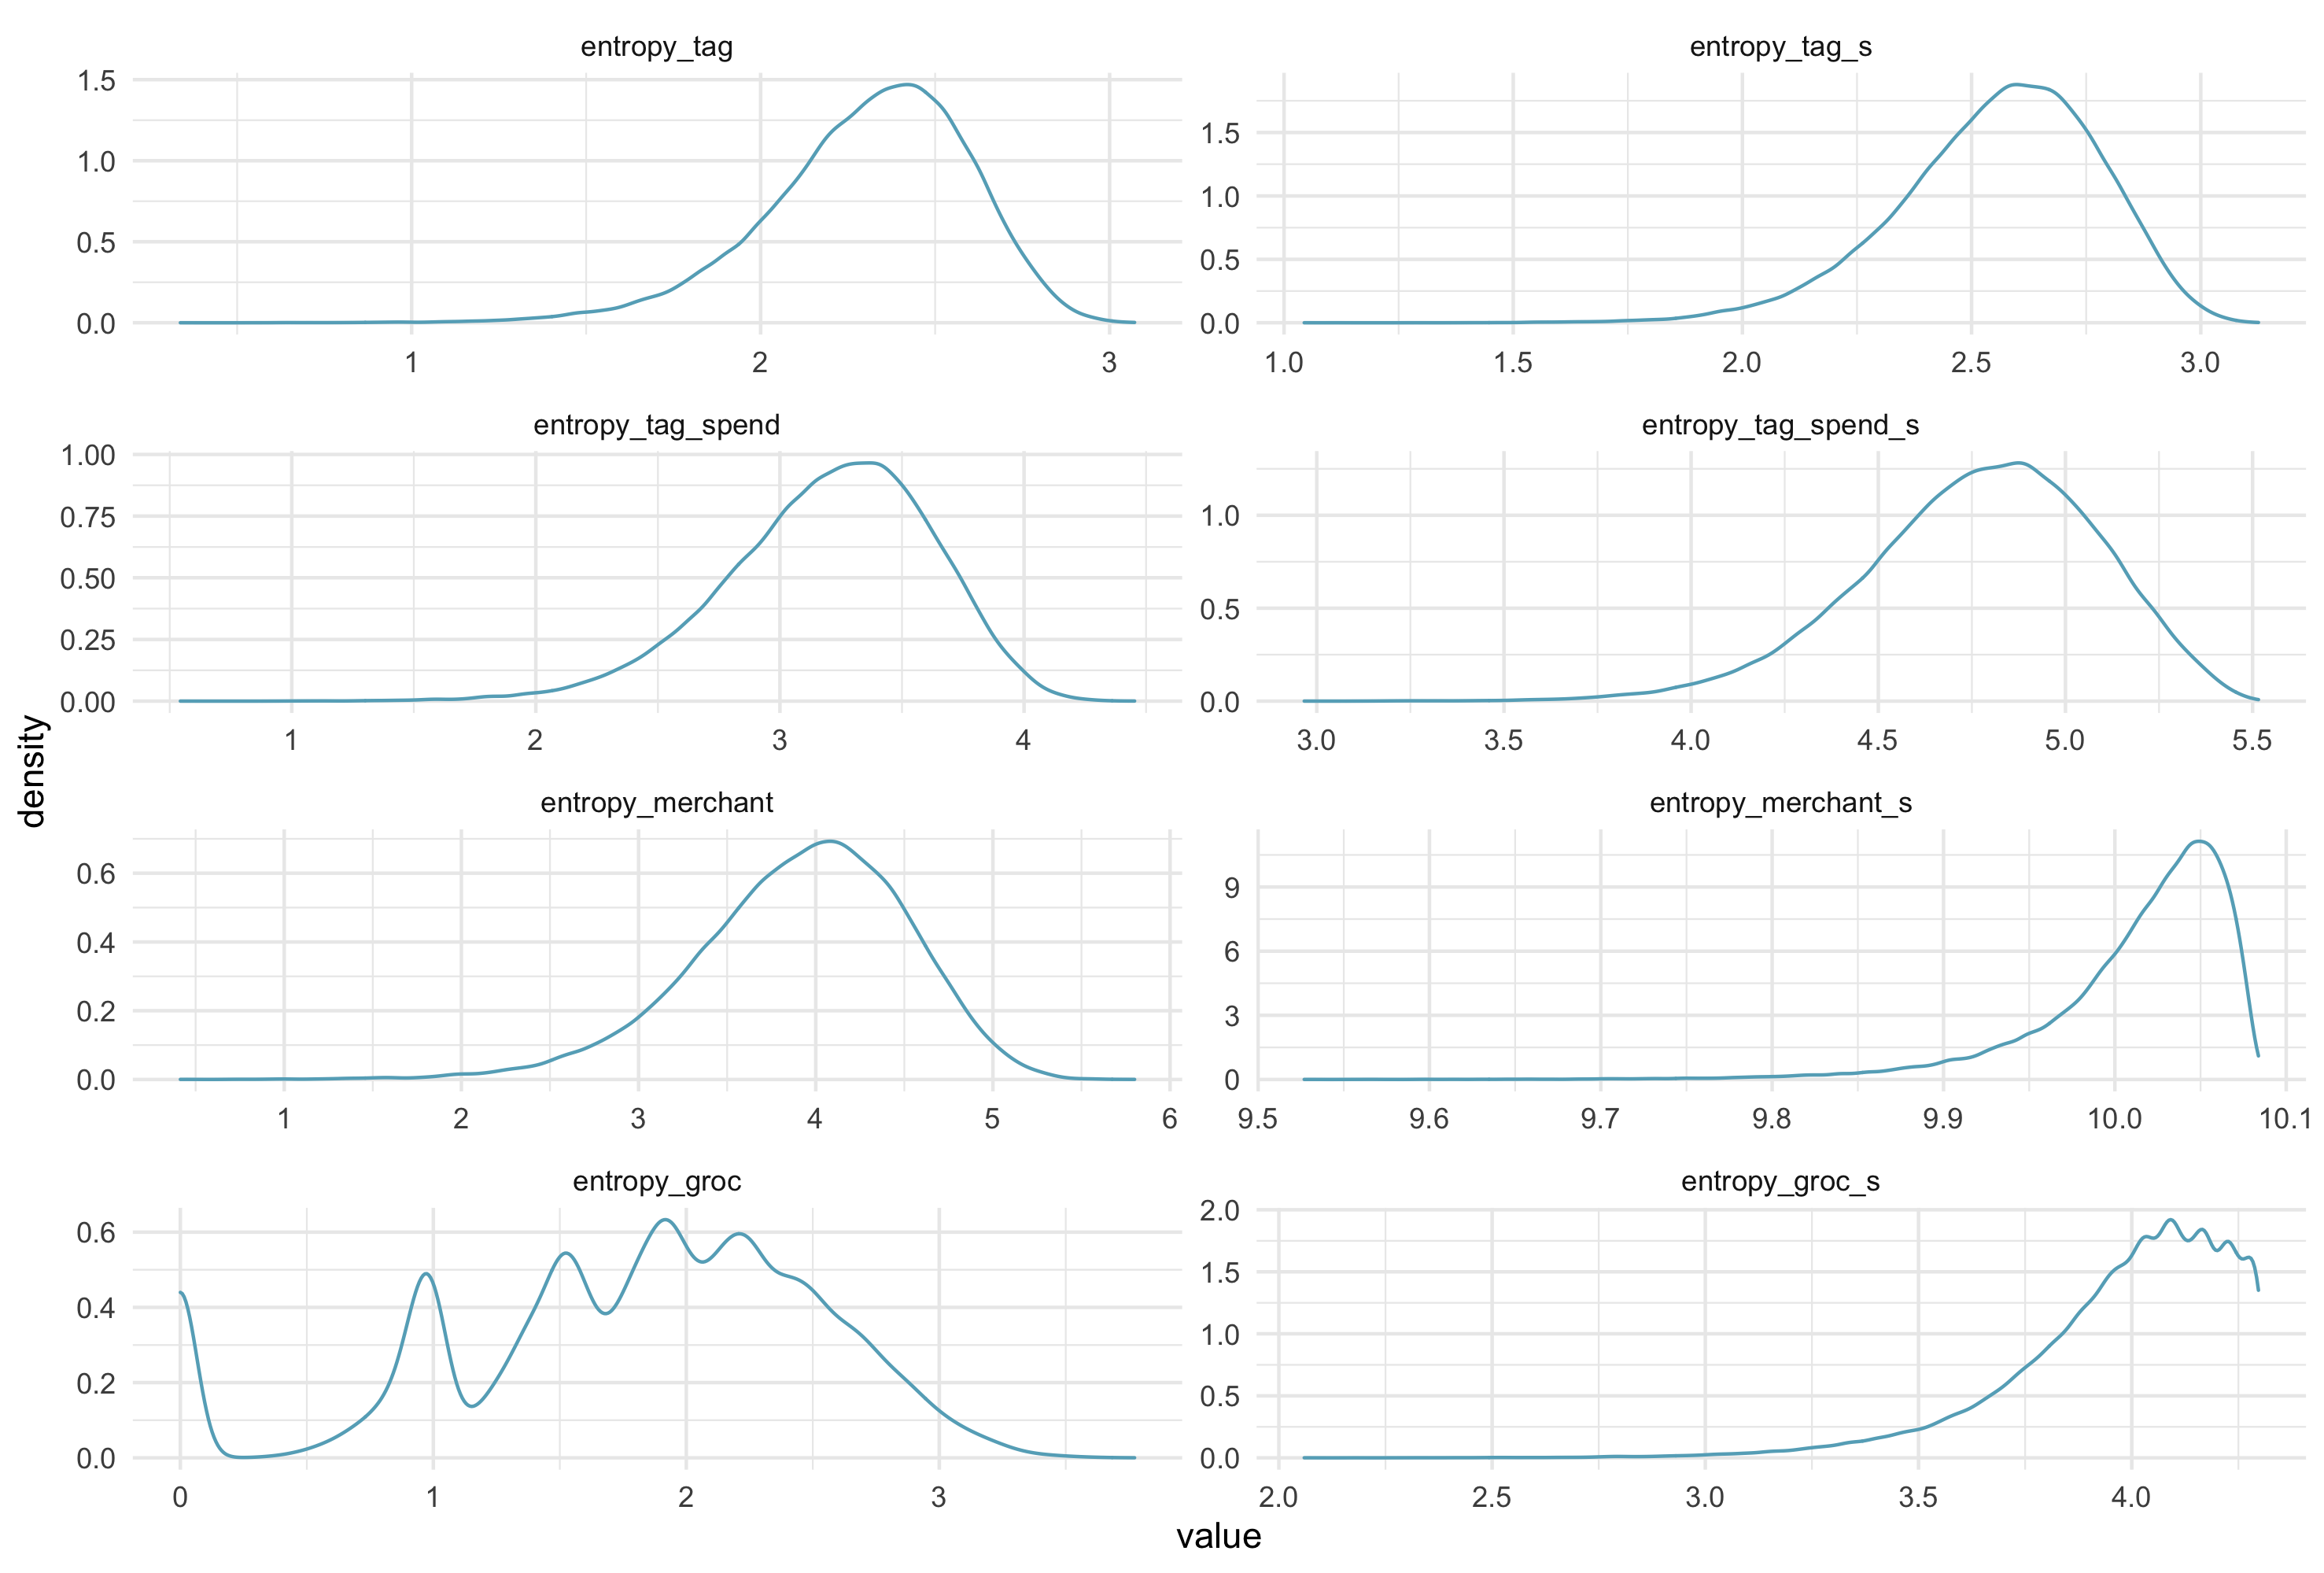
\includegraphics[width=\width]{\figdir/entropy_kdes.png}
    \fignote{\width}{}
\end{figure}




\subsection{Model specification}%
\label{par:model_specification}

We estimate models of the form: 

\begin{equation}
    s_{i,t} = \alpha_i + \lambda_t + \beta H_{i,t} + x^\prime_{i,t} \delta +
    \epsilon_{i,t},
\end{equation}

where $s_{i,t}$ is an indicator variable equal to one if individual $i$ made
one or more transfers to any of their savings account in month $t$ and zero
otherwise, $H_{it}$ is $i$'s spending entropy in month $t$, $x_{i,t}$ a vector
of control variables, $\alpha_i$ an individual fixed effect, $\lambda_t$ a
calendar month fixed effect, and $\epsilon_{i, t}$ the error term.

Issues to think about:
\begin{itemize}
    \item Unbalanced panel is not random - people using MDB for longer are
        different. Should we just use first x months for every user? E.g. first
        year?
\end{itemize}



% % !TEX root = ../entropy.tex

\section{Spending profiles}%
\label{sec:spending_profiles}

% Figure~\ref{fig:spending}
% \begin{figure}[H]
%     \center \newcommand\width{\textwidth} \caption{Spending behaviour}
%     \label{fig:spending}
%     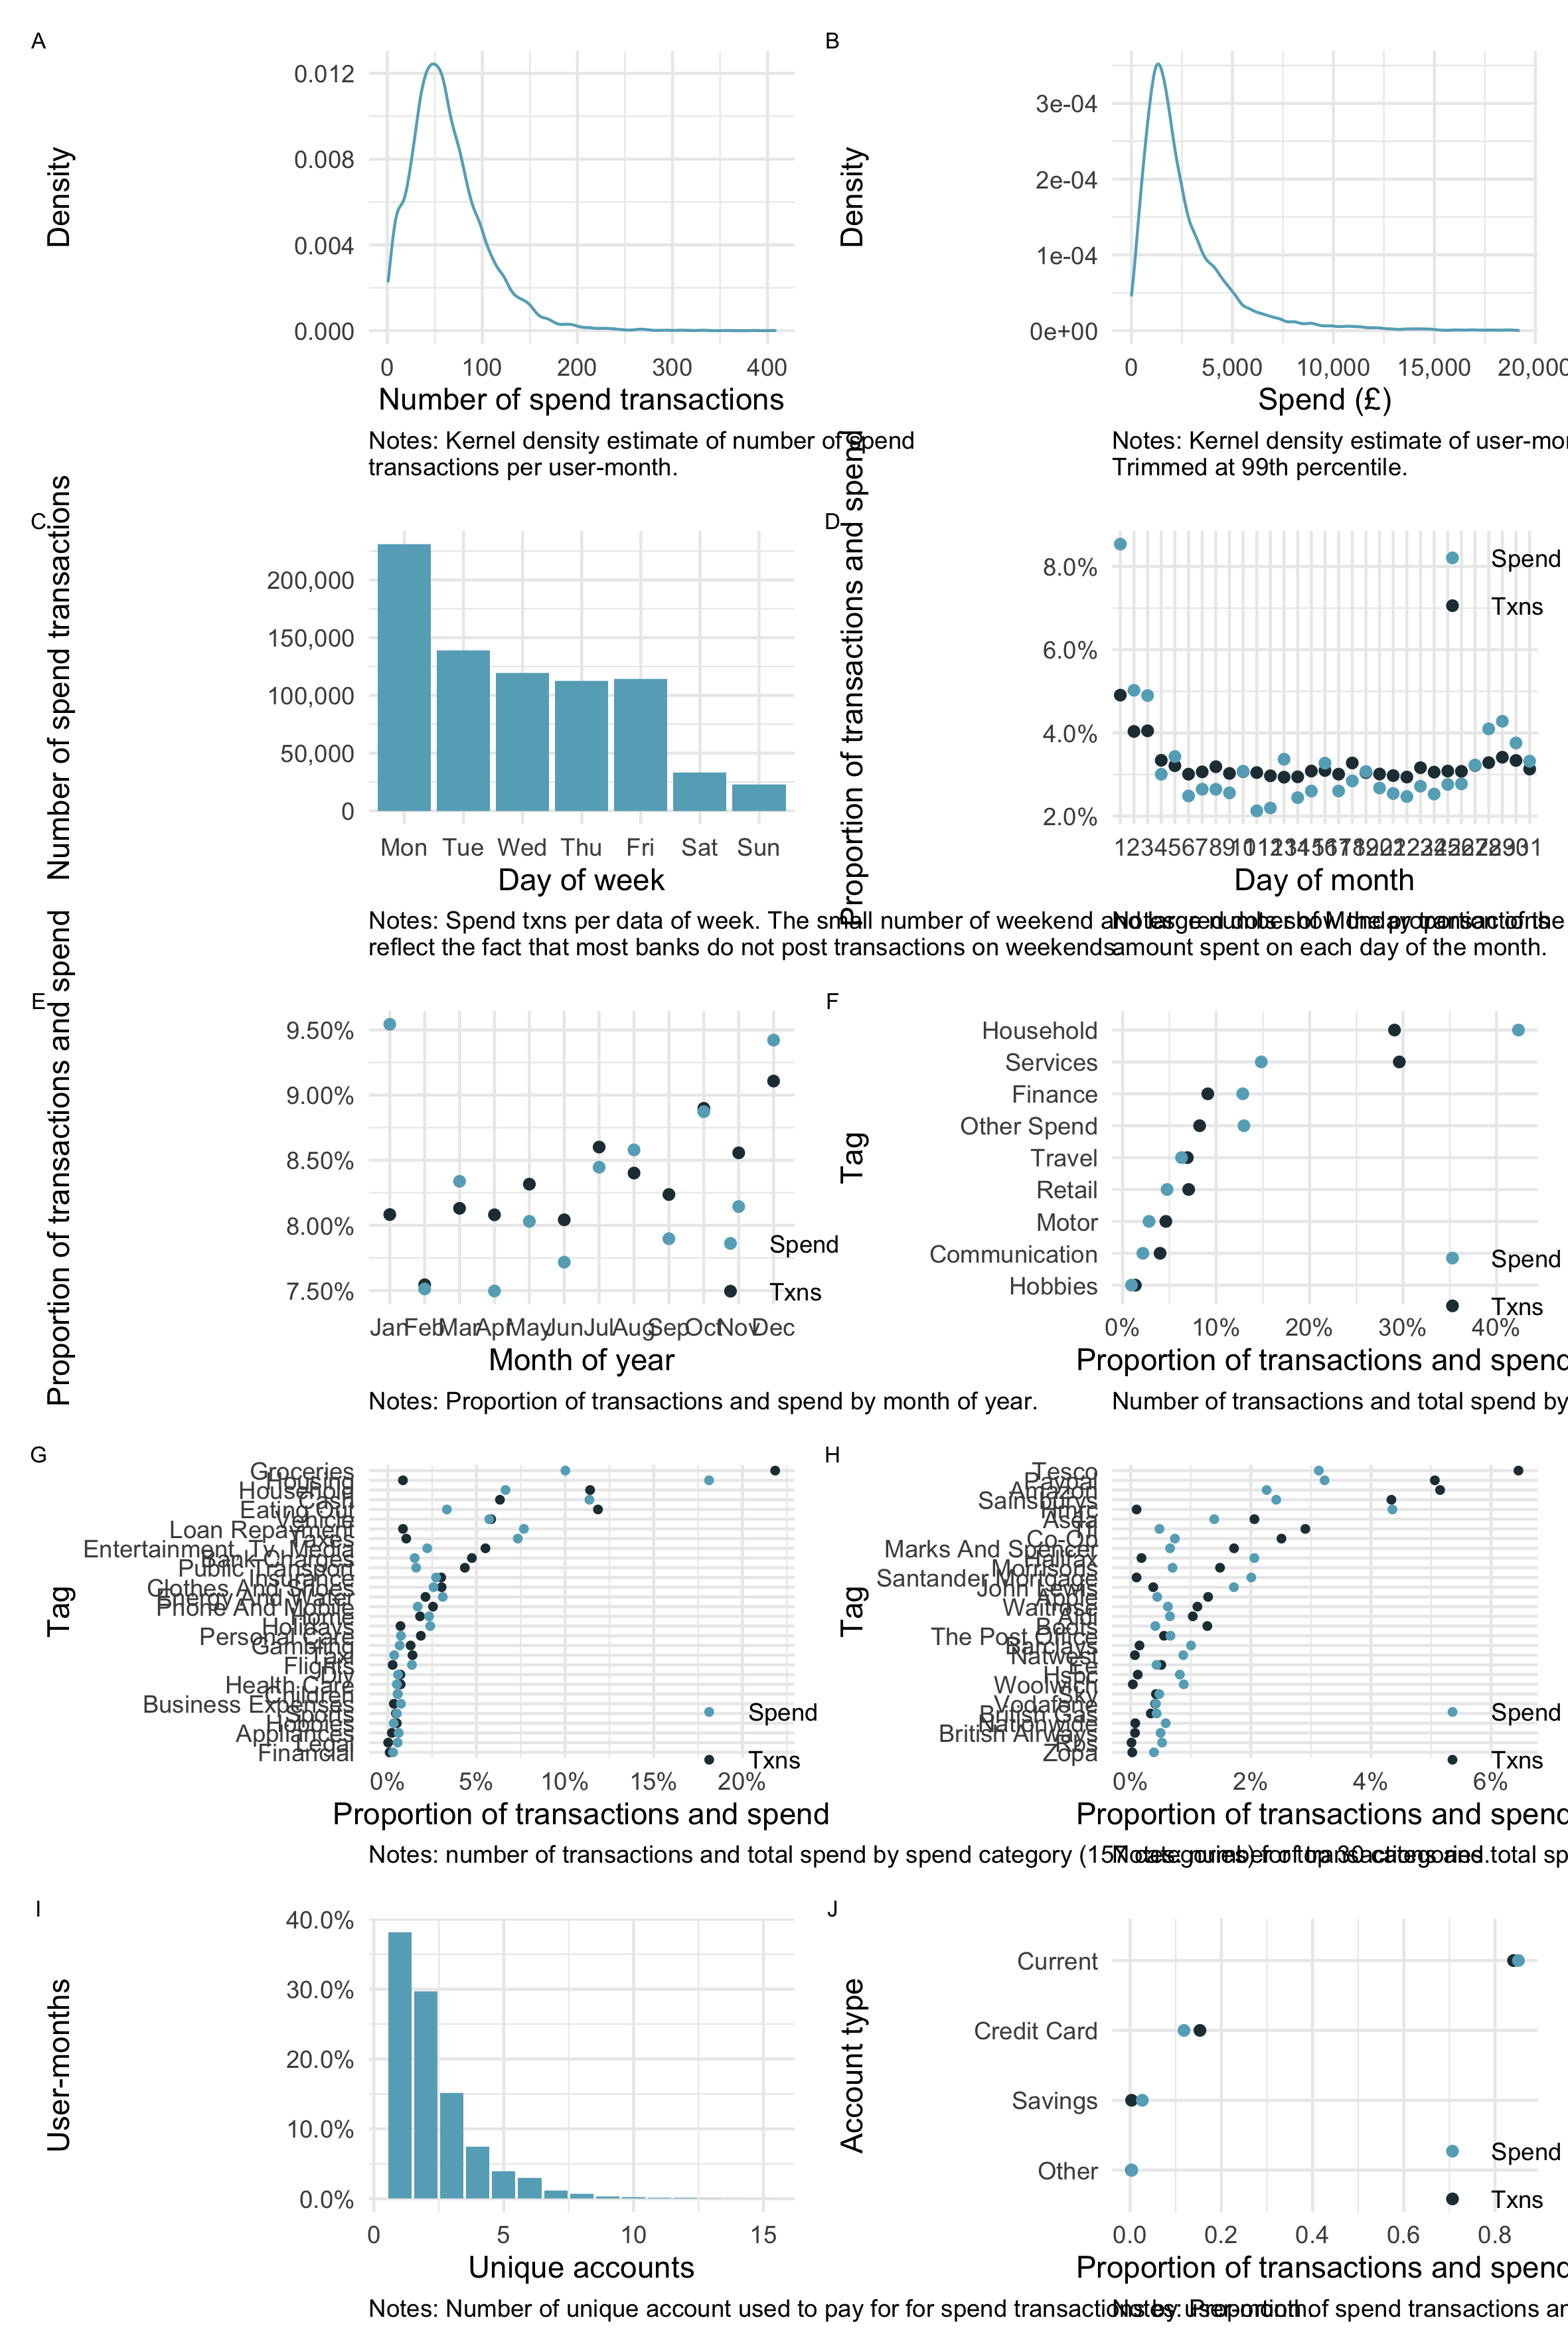
\includegraphics[width=\width]{\figdir/spending.png}
% \end{figure}





% % !TEX root = ../entropy.tex

\section{Savings patterns}%
\label{sec:savings_patterns}

survey examples
%https://www.mckinsey.com/capabilities/growth-marketing-and-sales/our-insights/how-us-consumers-are-feeling-shopping-and-spending-and-what-it-means-for-companies
%https://www.bls.gov/cex/

based on debit card data:
%https://www.barclayscorporate.com/insights/industry-expertise/uk-consumer-spending-report/
%https://www.ons.gov.uk/peoplepopulationandcommunity/personalandhouseholdfinances/expenditure/bulletins/familyspendingintheuk/april2019tomarch2020

% \begin{figure}[H]
%     \center \newcommand\width{\textwidth} \caption{Savings behaviour}
%     \label{fig:savings}
%     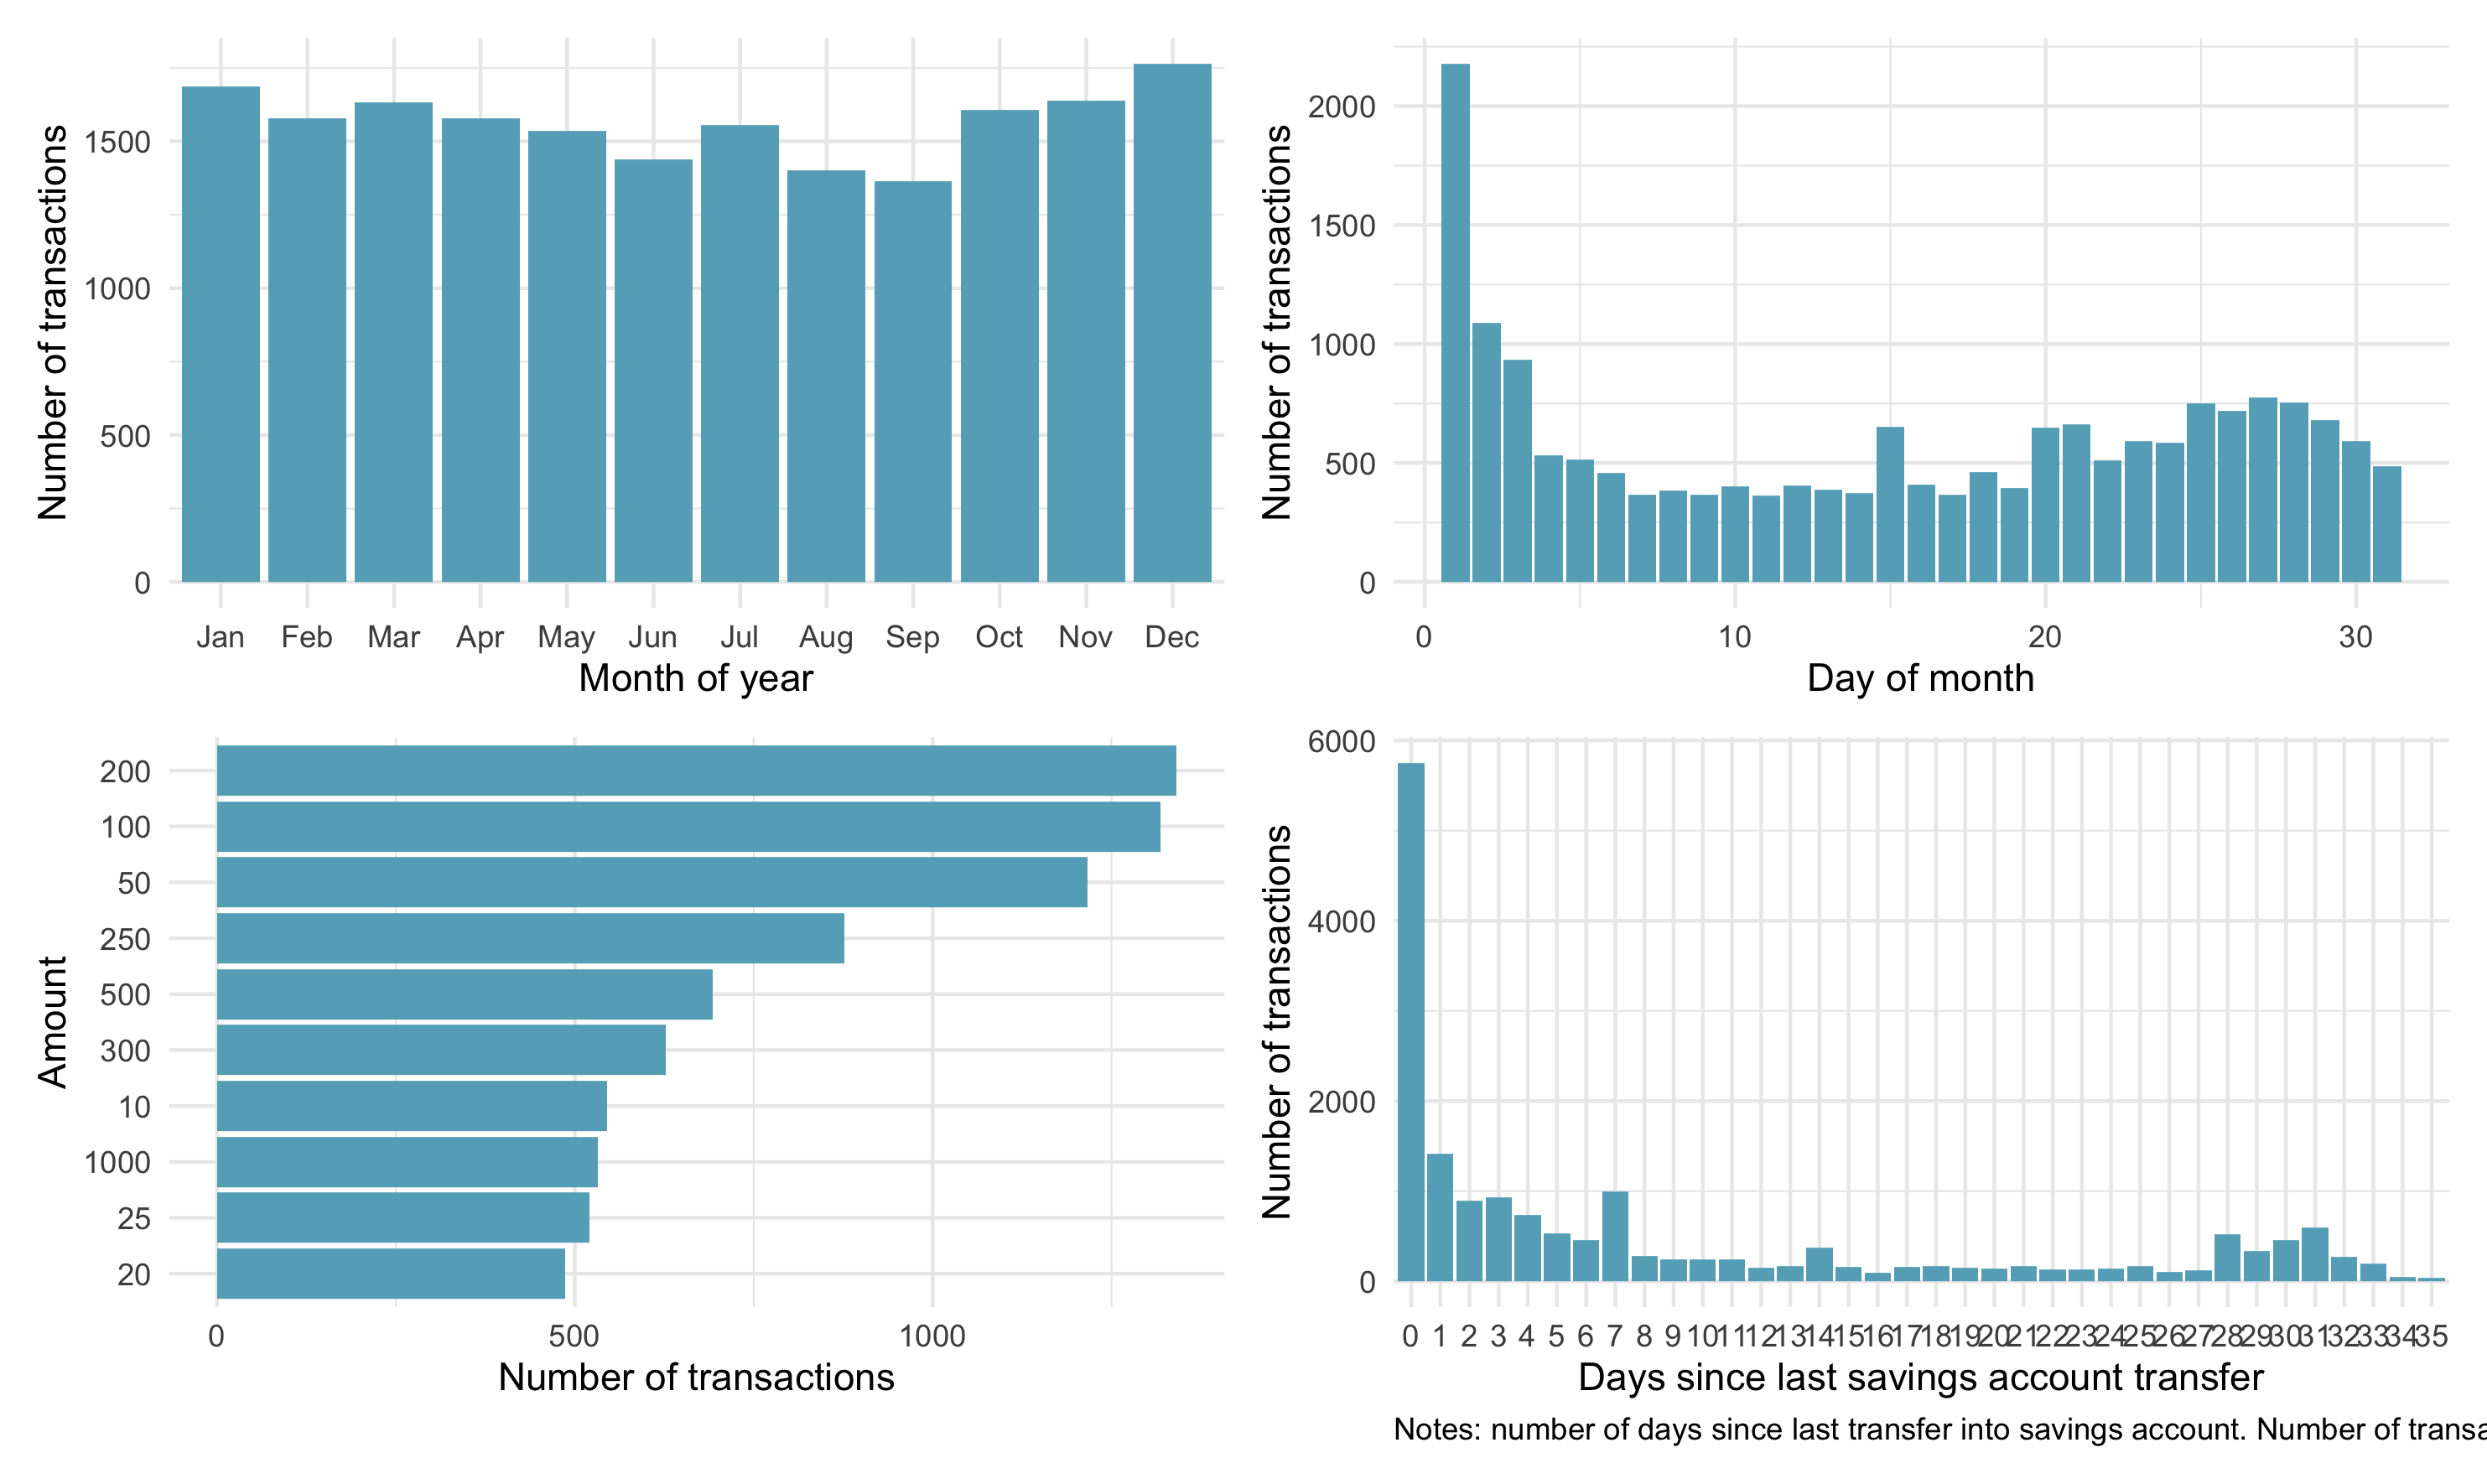
\includegraphics[width=\width]{\figdir/savings.png}
% \end{figure}



% !TEX root = ../entropy.tex

\section{Spending profiles predict emergency savings}%
\label{sec:results}

Table~\ref{tab:main} shows the effect of entropy on the probability of building
emergency savings in a given month. Columns (1)-(3) show results for unsmoothed
entropy based on 9 categories, 48 categories, and merchant names, respectively.
Columns (4)-(6) show results for smoothed entropy based on the same variables.
All models include user and year-month fixed effects, and standard errors are
clustered at the user-level. 95\% confidence intervals are shown in
brackets.\footnote{In line with an emerging consensus for how to avoid
    over-reliance on statistical significance, we deliberately do not show
    significance stars in our regression tables and instead emphasise the
    implications of the bounds of the confidence intervals when discussing our
    results. For two recent discussions, see \citet{imbens2021statistical,
romer2020praise}.}

Results for unsmoothed entropy suggest that a one standard-deviation increase
in spending entropy is associated with an increase in the probability of a user
making at least one transfer into their savings accounts of between 1.1 and 2.3
percentage points -- an effect equal to an increase in monthly income of
between \pounds1000 and \pounds2000. Combined, the results in the three columns
present very strong evidence that entropy captures something about users's
spending distribution that is related to their likelihood for making payments
into their savings accounts. Furthermore, entropy variables defined based on a
larger number of unique categories, that allow for a more precise segmentation
of spending behaviour, capture features of spending behaviour that are as
strongly or more strongly related to savings behaviour as monthly income.

The results for smoothed entropy are similar but a tend to be smaller in
magnitude, and -- together -- also provide strong evidence that smoothed
entropy captures features of spending behaviour that is related to savings
behaviour in a statistically significant and economically relevant way. The
main difference to the results for unsmoothed entropy is the reversal of the
sign of the coefficients: across all three measures, an increase in entropy is
estimated to be associated with a decrease in the likelihood of any savings
transactions. The effect of the measure based on 9 categories is not
meaningfully different from zero, but the estimates for the measures based on
48 categories and merchants are almost identical and suggest that the magnitude
of the effect is between 1.2 and 2.1 percentage points -- equalling the effect
of a reduction of monthly income of between \pounds1000 and \pounds2000.

\begin{landscape}
    \begin{table}[ht]
        \centering\scriptsize
        \caption{Effect of entropy on P(savings transactions)}
        \label{tab:main}
        
\begin{table}[htbp]
   \centering
   \tiny
   \begin{threeparttable}[b]
      \caption{\label{tab:reg_has_inflows_main} Effect of entropy on P(transfer into savings accounts)}
      \begin{tabular}{lcccccc}
         \tabularnewline \midrule \midrule
         Model:                     & (1)             & (2)             & (3)             & (4)              & (5)              & (6)\\  
         \midrule
         \emph{Variables}\\
         Entropy (9 cats)           & 0.016$^{***}$   &                 &                 &                  &                  &   \\   
                                    & [0.013; 0.019]  &                 &                 &                  &                  &   \\   
         Entropy (48 cats)          &                 & 0.029$^{***}$   &                 &                  &                  &   \\   
                                    &                 & [0.025; 0.033]  &                 &                  &                  &   \\   
         Entropy (merchant)         &                 &                 & 0.032$^{***}$   &                  &                  &   \\   
                                    &                 &                 & [0.029; 0.036]  &                  &                  &   \\   
         Entropy (9 cats, smooth)   &                 &                 &                 & -0.008$^{***}$   &                  &   \\   
                                    &                 &                 &                 & [-0.010; -0.006] &                  &   \\   
         Entropy (48 cats, smooth)  &                 &                 &                 &                  & -0.023$^{***}$   &   \\   
                                    &                 &                 &                 &                  & [-0.025; -0.020] &   \\   
         Entropy (merchant, smooth) &                 &                 &                 &                  &                  & -0.019$^{***}$\\   
                                    &                 &                 &                 &                  &                  & [-0.021; -0.016]\\   
         Month spend                & 0.009$^{***}$   & 0.009$^{***}$   & 0.008$^{***}$   & 0.009$^{***}$    & 0.008$^{***}$    & 0.007$^{***}$\\   
                                    & [0.009; 0.010]  & [0.008; 0.009]  & [0.008; 0.009]  & [0.009; 0.010]   & [0.007; 0.009]   & [0.007; 0.008]\\   
         Month income               & 0.012$^{***}$   & 0.012$^{***}$   & 0.012$^{***}$   & 0.012$^{***}$    & 0.011$^{***}$    & 0.011$^{***}$\\   
                                    & [0.011; 0.013]  & [0.011; 0.013]  & [0.011; 0.013]  & [0.011; 0.013]   & [0.011; 0.012]   & [0.010; 0.012]\\   
         Has income in month        & 0.086$^{***}$   & 0.084$^{***}$   & 0.083$^{***}$   & 0.087$^{***}$    & 0.085$^{***}$    & 0.086$^{***}$\\   
                                    & [0.077; 0.094]  & [0.075; 0.092]  & [0.074; 0.091]  & [0.079; 0.096]   & [0.076; 0.093]   & [0.078; 0.095]\\   
         Income variability         & 0.001$^{*}$     & 0.001$^{*}$     & 0.001$^{*}$     & 0.001$^{*}$      & 0.001$^{*}$      & 0.000\\   
                                    & [-0.000; 0.001] & [-0.000; 0.001] & [-0.000; 0.001] & [-0.000; 0.001]  & [-0.000; 0.001]  & [-0.000; 0.001]\\   
         \midrule
         \emph{Fixed-effects}\\
         User                       & Yes             & Yes             & Yes             & Yes              & Yes              & Yes\\  
         Year-month                 & Yes             & Yes             & Yes             & Yes              & Yes              & Yes\\  
         \midrule
         \emph{Fit statistics}\\
         Observations               & 1,043,727       & 1,043,727       & 1,043,416       & 1,043,727        & 1,043,727        & 1,043,416\\  
         R$^2$                      & 0.45368         & 0.45395         & 0.45410         & 0.45363          & 0.45415          & 0.45410\\  
         Within R$^2$               & 0.00719         & 0.00768         & 0.00807         & 0.00709          & 0.00805          & 0.00808\\  
         \midrule \midrule
         \multicolumn{7}{l}{\emph{Clustered (User) co-variance matrix, 95\% confidence intervals in brackets}}\\
         \multicolumn{7}{l}{\emph{Signif. Codes: ***: 0.01, **: 0.05, *: 0.1}}\\
      \end{tabular}
   \end{threeparttable}
\end{table}



        \tabnote{1.2\textwidth}{Results from estimating
            Equation~\ref{equ:model}. The
                dependent variable in all columns is a dummy variable
                indicating whether a
                    user made at least one transaction into any of their
                    savings accounts in a
                given period. \regtabinfo}
    \end{table}
\end{landscape}

As discussed in Section~\ref{sub:estimation}, these results are not due to
reverse causality. While we might think that making a savings transactions
might change some or all of the components of entropy discussed in
Section~\ref{sub:spending_profiles} -- the number of unique spending categories
with positive frequency count, the standard deviation of these counts, and the
total number of spend transactions -- and thus change entropy, this is not the
case because of the way we define entropy and savings, and the way spending
transactions are categorised. We define entropy based on all current account
debits that are identified as spends, while we define savings transactions as
the sum of all savings accounts credits. If a user transfers money from their
current account to their savings account, this will be identified as a savings
transaction, but be identified as a transfer on their current account and thus
not considered when calculating their entropy score.

The estimates of our control variables are largely as expected, with the
exception of monthly spend, which one might have expected to be negatively
correlated with savings. Also, it is evident that the strongest predictor among
the included controls for whether a user makes any savings transfer is whether
they receive any income in that month. Income variability, in contrast, is not
correlated with savings behaviour in any economically significant way,
suggesting that people with variable incomes do not build savings cushions for
periods where they have no income.

Overall, the effect of entropy in spending profiles is statistically and
economically significant, and robust across different definitions. In other
words, the scores seem to pick up a feature of the spending distribution that
is predictive of savings behaviour. The obvious question raised by the results
is why smoothing entropy scores flips the direction of the effect of entropy.
We address this next.


\subsection{Why does smoothing flip the direction of the effect}%
\label{sub:why_does_smoothing_flip_the_direction_of_the_effect}

One way to think about the sign change in Table~\ref{tab:main} is to realise
that it implies that at least for some individuals, the relative rank of
smoothed and unsmoothed entropy must differ considerably -- there must be some
individuals that have low unsmoothed entropy but high smoothed entropy or some
that have high unsmoothed entropy and low smoothed entropy or both.
Understanding who those individuals are might thus help us understand the sign
flip.

To understand rank differences between unsmoothed and smoothed entropy scores
it is useful to rewrite Equation~\ref{equ:entropy} in a way that makes it easy
to see its component parts. Remember from Section~\ref{sub:spending_profiles}
that $f_c$ is the number of transactions made by a user in a given period in
spending category $c$, $\setc$ the set of all spending categories, and $F$ the
total number of transactions made by a given user in a given period.
Additionally, let $\setcp = \{c: f_c > 0\}$ be the set of all spending
categories with positive frequency counts (i.e.  with at least one transaction)
and $\setcz = \{c: f_c = 0\}$ the set of all spending categories with a zero
frequency count, so that $\setc = \setcz \cup \setcp$. Then, using our
definitions of unsmoothed and smoothed probabilities, we can write unsmoothed
entropy as

\begin{equation}
\label{equ:entropy_us}
H = -\sum_{c \in \setcp}{\left(\frac{f_c}{F}\right)
log\left(\frac{f_c}{F}\right)},
\end{equation}

and smoothed entropy as:

\begin{equation}
\label{equ:entropy_s}
H^s = -\sum_{c \in \setcp}{\left(\frac{f_c + 1}{F + |\setc|}\right)
log\left(\frac{f_c + 1}{F + |\setc|}\right)}
- |\setcz|\left(\frac{1}{F + |\setc|}\right)
log\left(\frac{1}{F + |\setc|}\right),
\end{equation}

\noindent where the size of set $\setcz$, $|\setcz|$, is the number of all
spending categories in which a user makes no transactions in the period.
These expressions make clear that, by definition, unsmoothed entropy is a
function of frequency counts of categories with positive counts only while
smoothed entropy has two parts: the sum over all additively smoothed frequency
counts of categories with positive counts, plus the same sum for additively
smoothed probabilities of categories with zero counts, which reduces to a
constant term that is multiplied by the number of such categories.

The expressions also make transparent the three main components of both types
of entropy that are determined by user behaviour. The first is the number of
spending categories with a non-zero frequency count, $|\setcp|$, which
determines the number of elements summed over in Equation~\ref{equ:entropy_us},
and partitions the categories into either contributing to the sum on the left
hand side of Equation~\ref{equ:entropy_s} or -- given that for an exogenously
fixed $|\setc|$, $|\setcz| = |\setc \backslash \setcp|$ -- to the constant term
on the right hand side. The second component is the variation of the frequency
counts, $f_c$, and the third component is the number of total spend
transactions, $F = \sum_{\setc}f_c$. Together, these two elements determine the probabilities
associated with a spend transaction occurring in a given category. The number
of total spending categories, $|\setc|$, also determines smoothed entropy and,
implicitly, also unsmoothed entropy since it ``scales'' the number of
categories with a positive frequency count, $|\setcp|$, as a given number of
spending transactions are categorised into finer or coarser categories. But it
is exogenously given and does not depend on user behaviour.

\begin{figure}[ht]
    \centering 
    \caption{Effect of smoothing on entropy}
    \label{fig:scatter_facets}
    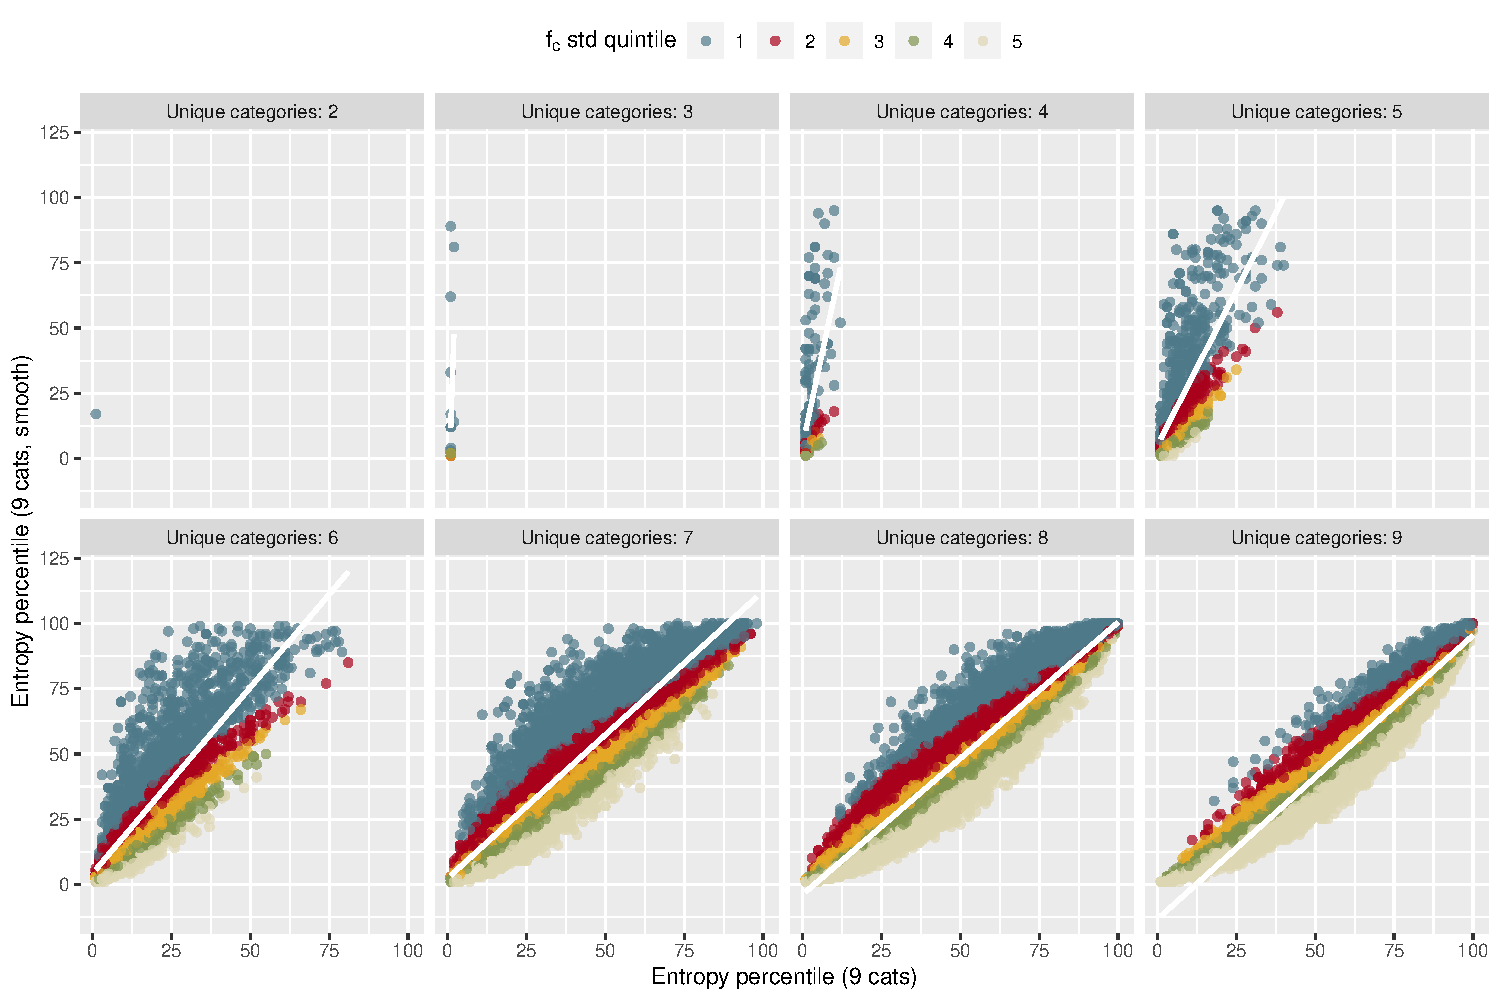
\includegraphics[width=\textwidth]{\figdir/scatter_facet_std_tag_q.pdf}
    \fignote{\textwidth}{Percentile ranks of 9-category-based unsmoothed and
    smoothed entropy separated by the number of categories with positive
frequency counts. White reference lines indicate equal percentile ranks;
colours, frequency count standard deviation quintiles. Figure is based on a
10\% sample of the dataset used for analysis. There are only 8 panels since
there are cases where a user has spends in only a single category.}
\end{figure}

These components help us reason about rank differences between unsmoothed and
smoothed entropy. From equations~\ref{equ:entropy_us} and~\ref{equ:entropy_s}
we can see that the first part of smoothed entropy that sums over all spending
categories with positive frequency counts is very similar to the entire
expression of unsmoothed entropy -- it is that same expression but with
additively smoothed probabilities. Hence, all else equal, the higher the number
of categories with positive counts, the more smoothed entropy is determined by
that first part, and the more similar it will be to unsmoothed entropy. As a
result, we would expect to find large (rank) differences between entropy scores
among cases with few positive-counts categories. Furthermore, given that
unsmoothed entropy is increasing in the number of categories with positive
counts, we expect these cases to have relatively low unsmoothed entropy.

Given that we expect high rank difference cases to make spends across a small
number of categories, and expect these cases to have low unsmoothed entropy,
high rank differences will occur among the subset of those cases that have high
smoothed entropy. Remember from Section~\ref{sub:spending_profiles} that
entropy is higher the more equal the spending category probabilities are.
Hence, for a given number of zero-count categories, smoothed entropy will be
higher if the (additively smoothed) probabilities of all positive-count
categories are close to the (additively smoothed) probabilities of the
zero-count categories, which will be the case (i) if there are few overall
transactions, such that frequency counts ($f_c$) are close to zero and (ii) if
the counts are similar.

Figure~\ref{fig:scatter_facets} visualises this entire line of reasoning for
our 9-category based entropy variable: it shows scatter plots of the percentile
ranks of unsmoothed and smoothed entropy with a reference line indicating
identical rank, separated by the number of categories with positive frequency
counts and coloured based on the quintile of the frequency count standard
deviation.\footnote{Colouring based on the quintile of the total number of
transactions leads to a very similar plot and is thus not shown.} First,
ignoring the colouring and focusing on the shape of the dots only we can see
that, as expected, the relationship between the two entropy measures is tighter
the higher the number of non-zero spending categories is. Cases with large
entropy rank differences are thus to be found among cases with fewer positive
spend categories. Among these, the colouring makes clear that, as expected, the
cases with the largest rank differences -- those with the furthest vertical
difference to the reference line -- have low variation in their frequency
counts. However, it is also clear that the reverse is not true: there are cases
with low count frequency variation that experience little or even a negative
rank difference. Furthermore, among cases with a higher number of categories
with positive counts, cases with a very high variation in frequency counts can
also experience quite large rank differences, albeit in the opposite direction.
Hence, while counts variation is some help in identifying cases with high
entropy rank differences, it does not do so perfectly.

One reason the relationship is not perfect is that while cases with few total
transactions that are evenly spread across a small number of categories will
have high smoothed entropy, such will also have high unsmoothed entropy. What
we are looking for, more precisely, are cases where this pattern holds broadly,
but that also have a small number of frequency counts that dominate the others
but are still relatively close to zero. This would lead to low unsmoothed
entropy (because of the dominant counts) but high smoothed entropy (because all
counts are still relatively close to zero, so that the additively smoothed
distribution resembles a uniform distribution). Further research will be
necessary to more fully classify such cases, and to inquire what it is about
their behaviour that might be related to savings behaviour.


\subsection{Is entropy informative beyond its component parts?}%
\label{sub:is_entropy_informative_beyond_its_component_parts_}

Another question that arises once we think of entropy as comprising three main
component parts is whether its non-linear nature captures anything about the
relationship between spending and saving behaviour that is not captured already
by the three simpler components. 

\begin{landscape}
\begin{table}[ht]
\centering\scriptsize
\caption{Controlling for components}
\label{tab:components}

\begin{table}[htbp]
   \centering
   \tiny
   \begin{threeparttable}[b]
      \caption{\label{tab:reg_has_inflows_comp} Controlling for entropy components}
      \begin{tabular}{lcccc}
         \tabularnewline \midrule \midrule
         Model:                    & (1)             & (2)             & (3)              & (4)\\  
         \midrule
         \emph{Variables}\\
         Entropy (48 cats)         & 0.029$^{***}$   & 0.013$^{***}$   &                  &   \\   
                                   & [0.025; 0.033]  & [0.006; 0.021]  &                  &   \\   
         Entropy (48 cats, smooth) &                 &                 & -0.023$^{***}$   & -0.028$^{***}$\\   
                                   &                 &                 & [-0.025; -0.020] & [-0.034; -0.022]\\   
         Unique categories         &                 & 0.004$^{***}$   &                  & 0.004$^{***}$\\   
                                   &                 & [0.003; 0.005]  &                  & [0.004; 0.005]\\   
         Category counts std.      &                 & 0.002           &                  & -0.015$^{***}$\\   
                                   &                 & [-0.001; 0.006] &                  & [-0.018; -0.011]\\   
         Number of spend txns      &                 & 0.000$^{***}$   &                  & 0.001$^{***}$\\   
                                   &                 & [0.000; 0.001]  &                  & [0.001; 0.001]\\   
         Month spend               & 0.009$^{***}$   & 0.005$^{***}$   & 0.008$^{***}$    & 0.005$^{***}$\\   
                                   & [0.008; 0.009]  & [0.004; 0.006]  & [0.007; 0.009]   & [0.005; 0.006]\\   
         Month income              & 0.012$^{***}$   & 0.011$^{***}$   & 0.011$^{***}$    & 0.011$^{***}$\\   
                                   & [0.011; 0.013]  & [0.010; 0.012]  & [0.011; 0.012]   & [0.010; 0.012]\\   
         Has income in month       & 0.084$^{***}$   & 0.079$^{***}$   & 0.085$^{***}$    & 0.078$^{***}$\\   
                                   & [0.075; 0.092]  & [0.070; 0.087]  & [0.076; 0.093]   & [0.070; 0.087]\\   
         Income variability        & 0.001$^{*}$     & 0.000           & 0.001$^{*}$      & 0.000\\   
                                   & [-0.000; 0.001] & [-0.000; 0.001] & [-0.000; 0.001]  & [-0.000; 0.001]\\   
         \midrule
         \emph{Fixed-effects}\\
         User                      & Yes             & Yes             & Yes              & Yes\\  
         Year-month                & Yes             & Yes             & Yes              & Yes\\  
         \midrule
         \emph{Fit statistics}\\
         Observations              & 1,043,727       & 1,043,727       & 1,043,727        & 1,043,727\\  
         R$^2$                     & 0.45395         & 0.45498         & 0.45415          & 0.45515\\  
         Within R$^2$              & 0.00768         & 0.00956         & 0.00805          & 0.00986\\  
         \midrule \midrule
         \multicolumn{5}{l}{\emph{Clustered (User) co-variance matrix, 95\% confidence intervals in brackets}}\\
         \multicolumn{5}{l}{\emph{Signif. Codes: ***: 0.01, **: 0.05, *: 0.1}}\\
      \end{tabular}
   \end{threeparttable}
\end{table}



\tabnote{1.5\textwidth}{\regtabinfo}
\end{table}
\end{landscape}

We can test this by checking whether the relationship between spending entropy
and the probability of making a savings transaction remains economically and
statistically significant once we control for the three components. Columns (1)
and (3) in Table~\ref{tab:components} replicate the results for the 48-category-based
unsmoothed and smoothed entropy measures presented in Table~\ref{tab:main} for
reference. In columns (2) and (4) we additionally control for the three entropy
components. Including these components has some effect: the coefficients change
slightly -- decreasing in absolute magnitude in the case of unsmoothed entropy,
increasing in the case of smoothed entropy -- while the width of the confidence
intervals about double in both cases, reflecting the strong collinearity amount
the component and entropy. However, both coefficients remain statistically
significant and their confidence intervals cover values that are also
economically significant. Hence, the results make clear that the results in
Table~\ref{tab:main} cannot be attributed simply to the effect of one or more
of entropy's simple components.





% % !TEX root = ../entropy.tex

\section{Discussion}%
\label{sec:discussion}

\edit{Ignore this section for now. Below are just notes.}
There are a number of alternative ways to characterise spend profiles. We could
calculate profiles based on the distribution of transaction values rather than
counts. We could also calculate profiles based on inter-temporal rather than
intra-temporal distributions, focusing on consistency of purchasing behaviour
over time rather than on predictability at any given time
\citep{krumme2013predictability}. Further, we could focus on time-based rather
than category-based measures, focusing, for instance, on whether purchases of
the same type tend to occur on the same day of the week
\citep{guidotti2015behavioral}. Finally, one could also create composite
measures based on principal component analysis, an approach used in
\citet{eagle2010network}. We leave these extensions for future research.



\newpage
\printbibliography
\newpage

\appendix

% % !TEX root = ../entropy.tex

\section{Interpreting entropy}%
\label{sec:interpreting_entropy}

To see how we can interpret entropy as the predictability of a user's spending
behaviour, it is useful to have a more complete understanding of
Equation~\ref{equ:entropy}. The building blocks of entropy is the information
content of a single event. The key intuition \citet{shannon1948mathematical}
aimed to capture was that learning of the occurrence of a low-probability event
is more informative than learning of the occurrence of a high-probability
event. The information of an event $I(E)$ is thus inversely proportional to is
probability $p(E)$. One way to capture this would be to define the information
of event E as $I(E) = \frac{1}{p(E)}$. Yet this implied that an event that is
certain to occur had information 1, when it would make sense to have
information 0. To remedy this (and also satisfy additional desireable
characteristics of an information function), Shannon proposed using the log of
the expression. Hence, the information of event E, often called \textit{Shannon
information}, \textit{self-information}, or just \textit{information}, is
defined as:

\begin{equation}
    I(E) = log\left(\frac{1}{p(E)}\right) = -log(p(E)).
\end{equation}

The choice of the base for the logarithm varies by application and determines
the units: base 2 means that information is expressed in bits; the natural
logarithm, another popular choice, expresses information in \textit{nats}.

Entropy, often called \textit{Information entropy}, \textit{Shannon entropy},
or just \textit{entropy}, is the information of a random variable, $X$, and
captures the expected amount of information of an event drawn at random from
the probability distribution of the random variable. It is calcualted as:

\begin{equation}
    H(X) = -\sum_x p(x) \times log(p(x)) = \sum_x p(x)I(x) = \mathbb{E} I(x).
\end{equation}

For a single event, the key intution was that the less likely an event, the
more information is conveyed when it occurs. The related idea for distributions
is similar: the less skewed a distribution of a random variable, the less
certain the realised value of a single draw from the distribution, the higher
is entropy - the maximum entropy distribution is the uniform distribution.




% !TEX root = ../entropy.tex

\section{Additional results}%
\label{sec:additional_results}

\subsection{Endogeneity}%
\label{sub:endogeneity}

As discussed in Section~\ref{sec:estimation}, one concern one might have about
our results in Section~\ref{sec:main_results} is reverse causality:
transferring money into savings accounts might change the distribution of spend
categories and thus change entropy. As noted previously, this is not a major
concern because of the way we calculate savings and spend profiles: savings are
calculated as the sum of inflows into savings accounts, while spend profiles
are based on the classification of spend transactions in current accounts, and
transfers from current to savings accounts are labelled as such and not treated
as spend transactions.

However, because transaction labelling is imperfect, it is possible that some
transfers are misclassified as spends and included in the calculation of
entropy scores. Two ways to deal with this is to use lagged entropy scores and
to explicitly control for the number of non-zero spend categories used to
calculate entropy scores. Here, we show that our results remain qualitatively
unchanged with both of these approaches.

Table~\ref{tab:reg_has_inflows_lag} presents results similar to the main
results in the main text, but using entropy lagged by one year-month period as
the independent variable of interest, while Table~\ref{tab:reg_has_inflows_cnz}
adds the number of non-zero spend categories as an additional control.

\def\yvars{has_inflows}
\foreach \y in \yvars {
    \input{\tabdir/reg_\y_cnz.tex}
    \input{\tabdir/reg_\y_lag.tex}
}


\subsection{Further results by financial resilience}%
\label{sub:results_by_financial_resilience}

The Tables below show results presented in
Section~\ref{sub:effect_of_financial_resilience} for alternative entropy
variables. 

\def\evars{entropy_tag, entropy_merchant}
\foreach \e in \evars {
    \input{\tabdir/reg_has_inflows_\e_z_inc_quint.tex}
    \input{\tabdir/reg_has_inflows_\e_sz_inc_quint.tex}
    \input{\tabdir/reg_has_inflows_\e_z_inc_var_quint.tex}
    \input{\tabdir/reg_has_inflows_\e_sz_inc_var_quint.tex}
}

% \subsection{Old stuff}%
% \label{sub:old_stuff}
% \newpage
% \subsection{Exploration}%
% \label{sub:exploration}
% 
\begin{table}[htbp]
   \centering
   \tiny
   \begin{threeparttable}[b]
      \caption{\label{tab:reg_has_sa_inflows_explore} Entropy exploration}
      \begin{tabular}{lccc}
         \tabularnewline \midrule \midrule
         Dependent Variable: & \multicolumn{3}{c}{Has savings}\\
         Model:                    & (1)             & (2)             & (3)\\  
         \midrule
         \emph{Variables}\\
         Entropy (48 cats)         &                 & 0.029$^{***}$   &   \\   
                                   &                 & [0.013; 0.044]  &   \\   
         Entropy (48 cats, smooth) &                 &                 & 0.004\\   
                                   &                 &                 & [-0.008; 0.016]\\   
         Spend txns                & 0.001$^{***}$   & 0.001$^{***}$   & 0.001$^{***}$\\   
                                   & [0.000; 0.001]  & [0.001; 0.001]  & [0.000; 0.001]\\   
         Unique categories         & 0.004$^{***}$   & 0.001           & 0.004$^{***}$\\   
                                   & [0.002; 0.006]  & [-0.002; 0.003] & [0.002; 0.006]\\   
         Paid with credit (\%)     & -0.000          & -0.000          & -0.000\\   
                                   & [-0.001; 0.000] & [-0.001; 0.000] & [-0.001; 0.000]\\   
         Month spend               & 0.006$^{***}$   & 0.005$^{***}$   & 0.006$^{***}$\\   
                                   & [0.003; 0.008]  & [0.003; 0.008]  & [0.003; 0.008]\\   
         Urban                     & -0.022          & -0.019          & -0.021\\   
                                   & [-0.230; 0.187] & [-0.230; 0.192] & [-0.230; 0.187]\\   
         Month income              & 0.000           & -0.000          & 0.000\\   
                                   & [-0.007; 0.007] & [-0.007; 0.006] & [-0.007; 0.007]\\   
         Has income in month       & 0.038$^{**}$    & 0.038$^{**}$    & 0.038$^{**}$\\   
                                   & [0.008; 0.068]  & [0.008; 0.068]  & [0.009; 0.068]\\   
         Income variability        & -0.003          & -0.003          & -0.003\\   
                                   & [-0.012; 0.006] & [-0.012; 0.005] & [-0.012; 0.005]\\   
         Rent payment              & 0.023$^{**}$    & 0.024$^{**}$    & 0.023$^{**}$\\   
                                   & [0.004; 0.043]  & [0.004; 0.043]  & [0.004; 0.043]\\   
         Mortgage payment          & 0.015           & 0.015           & 0.015\\   
                                   & [-0.009; 0.039] & [-0.009; 0.039] & [-0.009; 0.039]\\   
         Loan repayment            & 0.003           & 0.003           & 0.003\\   
                                   & [-0.013; 0.019] & [-0.012; 0.019] & [-0.013; 0.019]\\   
         Benefits                  & -0.010          & -0.011          & -0.010\\   
                                   & [-0.048; 0.028] & [-0.049; 0.027] & [-0.048; 0.028]\\   
         \midrule
         \emph{Fixed-effects}\\
         User id                   & Yes             & Yes             & Yes\\  
         Calendar month            & Yes             & Yes             & Yes\\  
         \midrule
         \emph{Fit statistics}\\
         Observations              & 83,935          & 83,935          & 83,935\\  
         R$^2$                     & 0.42912         & 0.42929         & 0.42913\\  
         Within R$^2$              & 0.00464         & 0.00494         & 0.00465\\  
         \midrule \midrule
         \multicolumn{4}{l}{\emph{Clustered (User id) co-variance matrix, 95\% confidence intervals in brackets}}\\
         \multicolumn{4}{l}{\emph{Signif. Codes: ***: 0.01, **: 0.05, *: 0.1}}\\
      \end{tabular}
      
      \begin{tablenotes}\footnotesize
         \item Notes: Spend and income variables are in \pounds'000.
      \end{tablenotes}
   \end{threeparttable}
\end{table}



\begin{table}[htbp]
   \centering
   \begin{threeparttable}[b]
      \caption{Components exploration}
      \begin{tabular}{lcccc}
         \tabularnewline \midrule \midrule
         Dependent Variable: & \multicolumn{4}{c}{Has savings}\\
         Model:                 & (1)             & (2)             & (3)              & (4)\\  
         \midrule
         \emph{Variables}\\
         Entropy (48 cats)      &                 & 0.032$^{***}$   &                  & 0.044$^{***}$\\   
                                &                 & [0.021; 0.042]  &                  & [0.024; 0.064]\\   
         Average spend          &                 &                 & 0.000$^{*}$      & 0.000$^{**}$\\   
                                &                 &                 & [-0.000; 0.000]  & [0.000; 0.000]\\   
         Cnz                    &                 &                 & 0.006$^{***}$    & 0.001\\   
                                &                 &                 & [0.004; 0.007]   & [-0.002; 0.003]\\   
         Counts std all         &                 &                 & 0.004$^{**}$     & 0.011$^{***}$\\   
                                &                 &                 & [0.001; 0.008]   & [0.006; 0.016]\\   
         Paid with credit (\%)  & -0.000          & -0.000          & -0.000$^{**}$    & -0.000$^{**}$\\   
                                & [-0.001; 0.000] & [-0.001; 0.000] & [-0.001; -0.000] & [-0.001; -0.000]\\   
         Month spend            & 0.020$^{***}$   & 0.019$^{***}$   & 0.015$^{***}$    & 0.014$^{***}$\\   
                                & [0.018; 0.023]  & [0.017; 0.022]  & [0.011; 0.019]   & [0.010; 0.018]\\   
         Urban                  & -0.039          & -0.037          & -0.037           & -0.036\\   
                                & [-0.230; 0.152] & [-0.234; 0.159] & [-0.233; 0.158]  & [-0.234; 0.163]\\   
         Month income           & 0.004           & 0.003           & 0.003            & 0.002\\   
                                & [-0.003; 0.011] & [-0.004; 0.010] & [-0.004; 0.009]  & [-0.005; 0.009]\\   
         Has income in month    & 0.039$^{**}$    & 0.037$^{**}$    & 0.032$^{**}$     & 0.031$^{*}$\\   
                                & [0.007; 0.071]  & [0.005; 0.069]  & [0.000; 0.064]   & [-0.000; 0.063]\\   
         Income variability     & 0.003           & 0.003           & 0.003            & 0.003\\   
                                & [-0.006; 0.012] & [-0.006; 0.012] & [-0.006; 0.011]  & [-0.006; 0.011]\\   
         Rent payment           & 0.028$^{***}$   & 0.025$^{***}$   & 0.023$^{**}$     & 0.023$^{**}$\\   
                                & [0.009; 0.047]  & [0.006; 0.043]  & [0.004; 0.041]   & [0.004; 0.042]\\   
         Mortgage payment       & 0.008           & 0.003           & -0.000           & -0.000\\   
                                & [-0.016; 0.033] & [-0.022; 0.027] & [-0.025; 0.024]  & [-0.025; 0.024]\\   
         Loan repayment         & 0.004           & -0.000          & -0.003           & -0.002\\   
                                & [-0.012; 0.020] & [-0.016; 0.016] & [-0.019; 0.013]  & [-0.018; 0.014]\\   
         Benefits               & -0.004          & -0.005          & -0.007           & -0.008\\   
                                & [-0.041; 0.033] & [-0.043; 0.032] & [-0.044; 0.030]  & [-0.045; 0.030]\\   
         \midrule
         \emph{Fixed-effects}\\
         User id                & Yes             & Yes             & Yes              & Yes\\  
         Calendar month         & Yes             & Yes             & Yes              & Yes\\  
         \midrule
         \emph{Fit statistics}\\
         Observations           & 91,644          & 91,644          & 91,644           & 91,644\\  
         R$^2$                  & 0.41730         & 0.41776         & 0.41807          & 0.41833\\  
         Within R$^2$           & 0.00782         & 0.00860         & 0.00914          & 0.00957\\  
         \midrule \midrule
         \multicolumn{5}{l}{\emph{Clustered (User id) co-variance matrix, 95\% confidence intervals in brackets}}\\
         \multicolumn{5}{l}{\emph{Signif. Codes: ***: 0.01, **: 0.05, *: 0.1}}\\
      \end{tabular}
   \end{threeparttable}
\end{table}



% 
\begin{table}[htbp]
   \centering
   \tiny
   \begin{threeparttable}[b]
      \caption{\label{tab:reg_has_sa_inflows_explore} Entropy exploration}
      \begin{tabular}{lccccc}
         \tabularnewline \midrule \midrule
         Dependent Variable: & \multicolumn{5}{c}{Entropy (48 cats)}\\
         Model:                    & (1)            & (2)            & (3)            & (4)              & (5)\\  
         \midrule
         \emph{Variables}\\
         Entropy (48 cats, smooth) & 0.274$^{***}$  &                &                &                  & 0.539$^{***}$\\   
                                   & [0.264; 0.285] &                &                &                  & [0.528; 0.550]\\   
         Spend txns                &                & 0.001$^{***}$  &                &                  & 0.010$^{***}$\\   
                                   &                & [0.001; 0.002] &                &                  & [0.010; 0.010]\\   
         Unique categories         &                &                & 0.097$^{***}$  &                  & 0.081$^{***}$\\   
                                   &                &                & [0.096; 0.099] &                  & [0.079; 0.082]\\   
         Category count variation  &                &                &                & -0.000$^{***}$   & -0.000$^{***}$\\   
                                   &                &                &                & [-0.000; -0.000] & [-0.000; -0.000]\\   
         \midrule
         \emph{Fixed-effects}\\
         User id                   & Yes            & Yes            & Yes            & Yes              & Yes\\  
         Calendar month            & Yes            & Yes            & Yes            & Yes              & Yes\\  
         \midrule
         \emph{Fit statistics}\\
         Observations              & 83,935         & 83,935         & 83,935         & 83,935           & 83,935\\  
         R$^2$                     & 0.66423        & 0.59311        & 0.77939        & 0.61808          & 0.92879\\  
         Within R$^2$              & 0.17916        & 0.00530        & 0.46067        & 0.06634          & 0.82592\\  
         \midrule \midrule
         \multicolumn{6}{l}{\emph{Clustered (User id) co-variance matrix, 95\% confidence intervals in brackets}}\\
         \multicolumn{6}{l}{\emph{Signif. Codes: ***: 0.01, **: 0.05, *: 0.1}}\\
      \end{tabular}
      
      \begin{tablenotes}\footnotesize
         \item Notes: Spend and income variables are in \pounds'000.
      \end{tablenotes}
   \end{threeparttable}
\end{table}



% 
\begin{table}[htbp]
   \centering
   \tiny
   \begin{threeparttable}[b]
      \caption{\label{tab:reg_has_sa_inflows_explore} Entropy exploration}
      \begin{tabular}{lccccc}
         \tabularnewline \midrule \midrule
         Dependent Variable: & \multicolumn{5}{c}{Entropy (48 cats)}\\
         Model:                    & (1)            & (2)            & (3)              & (4)              & (5)\\  
         \midrule
         \emph{Variables}\\
         Entropy (48 cats, smooth) & 0.212$^{***}$  &                &                  &                  & 0.530$^{***}$\\   
                                   & [0.208; 0.216] &                &                  &                  & [0.526; 0.533]\\   
         Spend txns                &                & 0.003$^{***}$  &                  &                  & 0.010$^{***}$\\   
                                   &                & [0.003; 0.003] &                  &                  & [0.010; 0.010]\\   
         Unique categories         &                &                & 0.098$^{***}$    &                  & 0.080$^{***}$\\   
                                   &                &                & [0.097; 0.098]   &                  & [0.080; 0.081]\\   
         Category count variation  &                &                &                  & -0.000$^{***}$   & -0.000$^{***}$\\   
                                   &                &                &                  & [-0.000; -0.000] & [-0.000; -0.000]\\   
         (Intercept)               & 0.501$^{***}$  & 0.213$^{***}$  & -1.079$^{***}$   & 0.508$^{***}$    & -1.228$^{***}$\\   
                                   & [0.497; 0.504] & [0.205; 0.221] & [-1.088; -1.069] & [0.503; 0.512]   & [-1.232; -1.223]\\   
         \midrule
         \emph{Fit statistics}\\
         Observations              & 83,935         & 83,935         & 83,935           & 83,935           & 83,935\\  
         R$^2$                     & 0.10447        & 0.04296        & 0.56104          & 0.02614          & 0.88513\\  
         Adjusted R$^2$            & 0.10446        & 0.04295        & 0.56104          & 0.02613          & 0.88513\\  
         \midrule \midrule
         \multicolumn{6}{l}{\emph{IID co-variance matrix, 95\% confidence intervals in brackets}}\\
         \multicolumn{6}{l}{\emph{Signif. Codes: ***: 0.01, **: 0.05, *: 0.1}}\\
      \end{tabular}
      
      \begin{tablenotes}\footnotesize
         \item Notes: Spend and income variables are in \pounds'000.
      \end{tablenotes}
   \end{threeparttable}
\end{table}



% % 
\begin{table}[htbp]
   \centering
   \tiny
   \begin{threeparttable}[b]
      \caption{\label{tab:reg_has_sa_inflows_explore} Entropy exploration}
      \begin{tabular}{lc}
         \tabularnewline \midrule \midrule
         Dependent Variable:       & Has savings\\  
         Model:                    & (1)\\  
         \midrule
         \emph{Variables}\\
         Entropy (48 cats, smooth) & -0.012$^{***}$\\   
                                   & [-0.016; -0.008]\\   
         (Intercept)               & 0.369$^{***}$\\   
                                   & [0.366; 0.373]\\   
         \midrule
         \emph{Fit statistics}\\
         Observations              & 83,935\\  
         R$^2$                     & 0.00040\\  
         Adjusted R$^2$            & 0.00039\\  
         \midrule \midrule
         \multicolumn{2}{l}{\emph{IID co-variance matrix, 95\% confidence intervals in brackets}}\\
         \multicolumn{2}{l}{\emph{Signif. Codes: ***: 0.01, **: 0.05, *: 0.1}}\\
      \end{tabular}
      
      \begin{tablenotes}\footnotesize
         \item Notes: Spend and income variables are in \pounds'000.
      \end{tablenotes}
   \end{threeparttable}
\end{table}




% \newpage
% \begin{figure}[H]
%     \caption{Diagnostics}
%     \label{fig:diagnostics}
%     \begin{center}
%         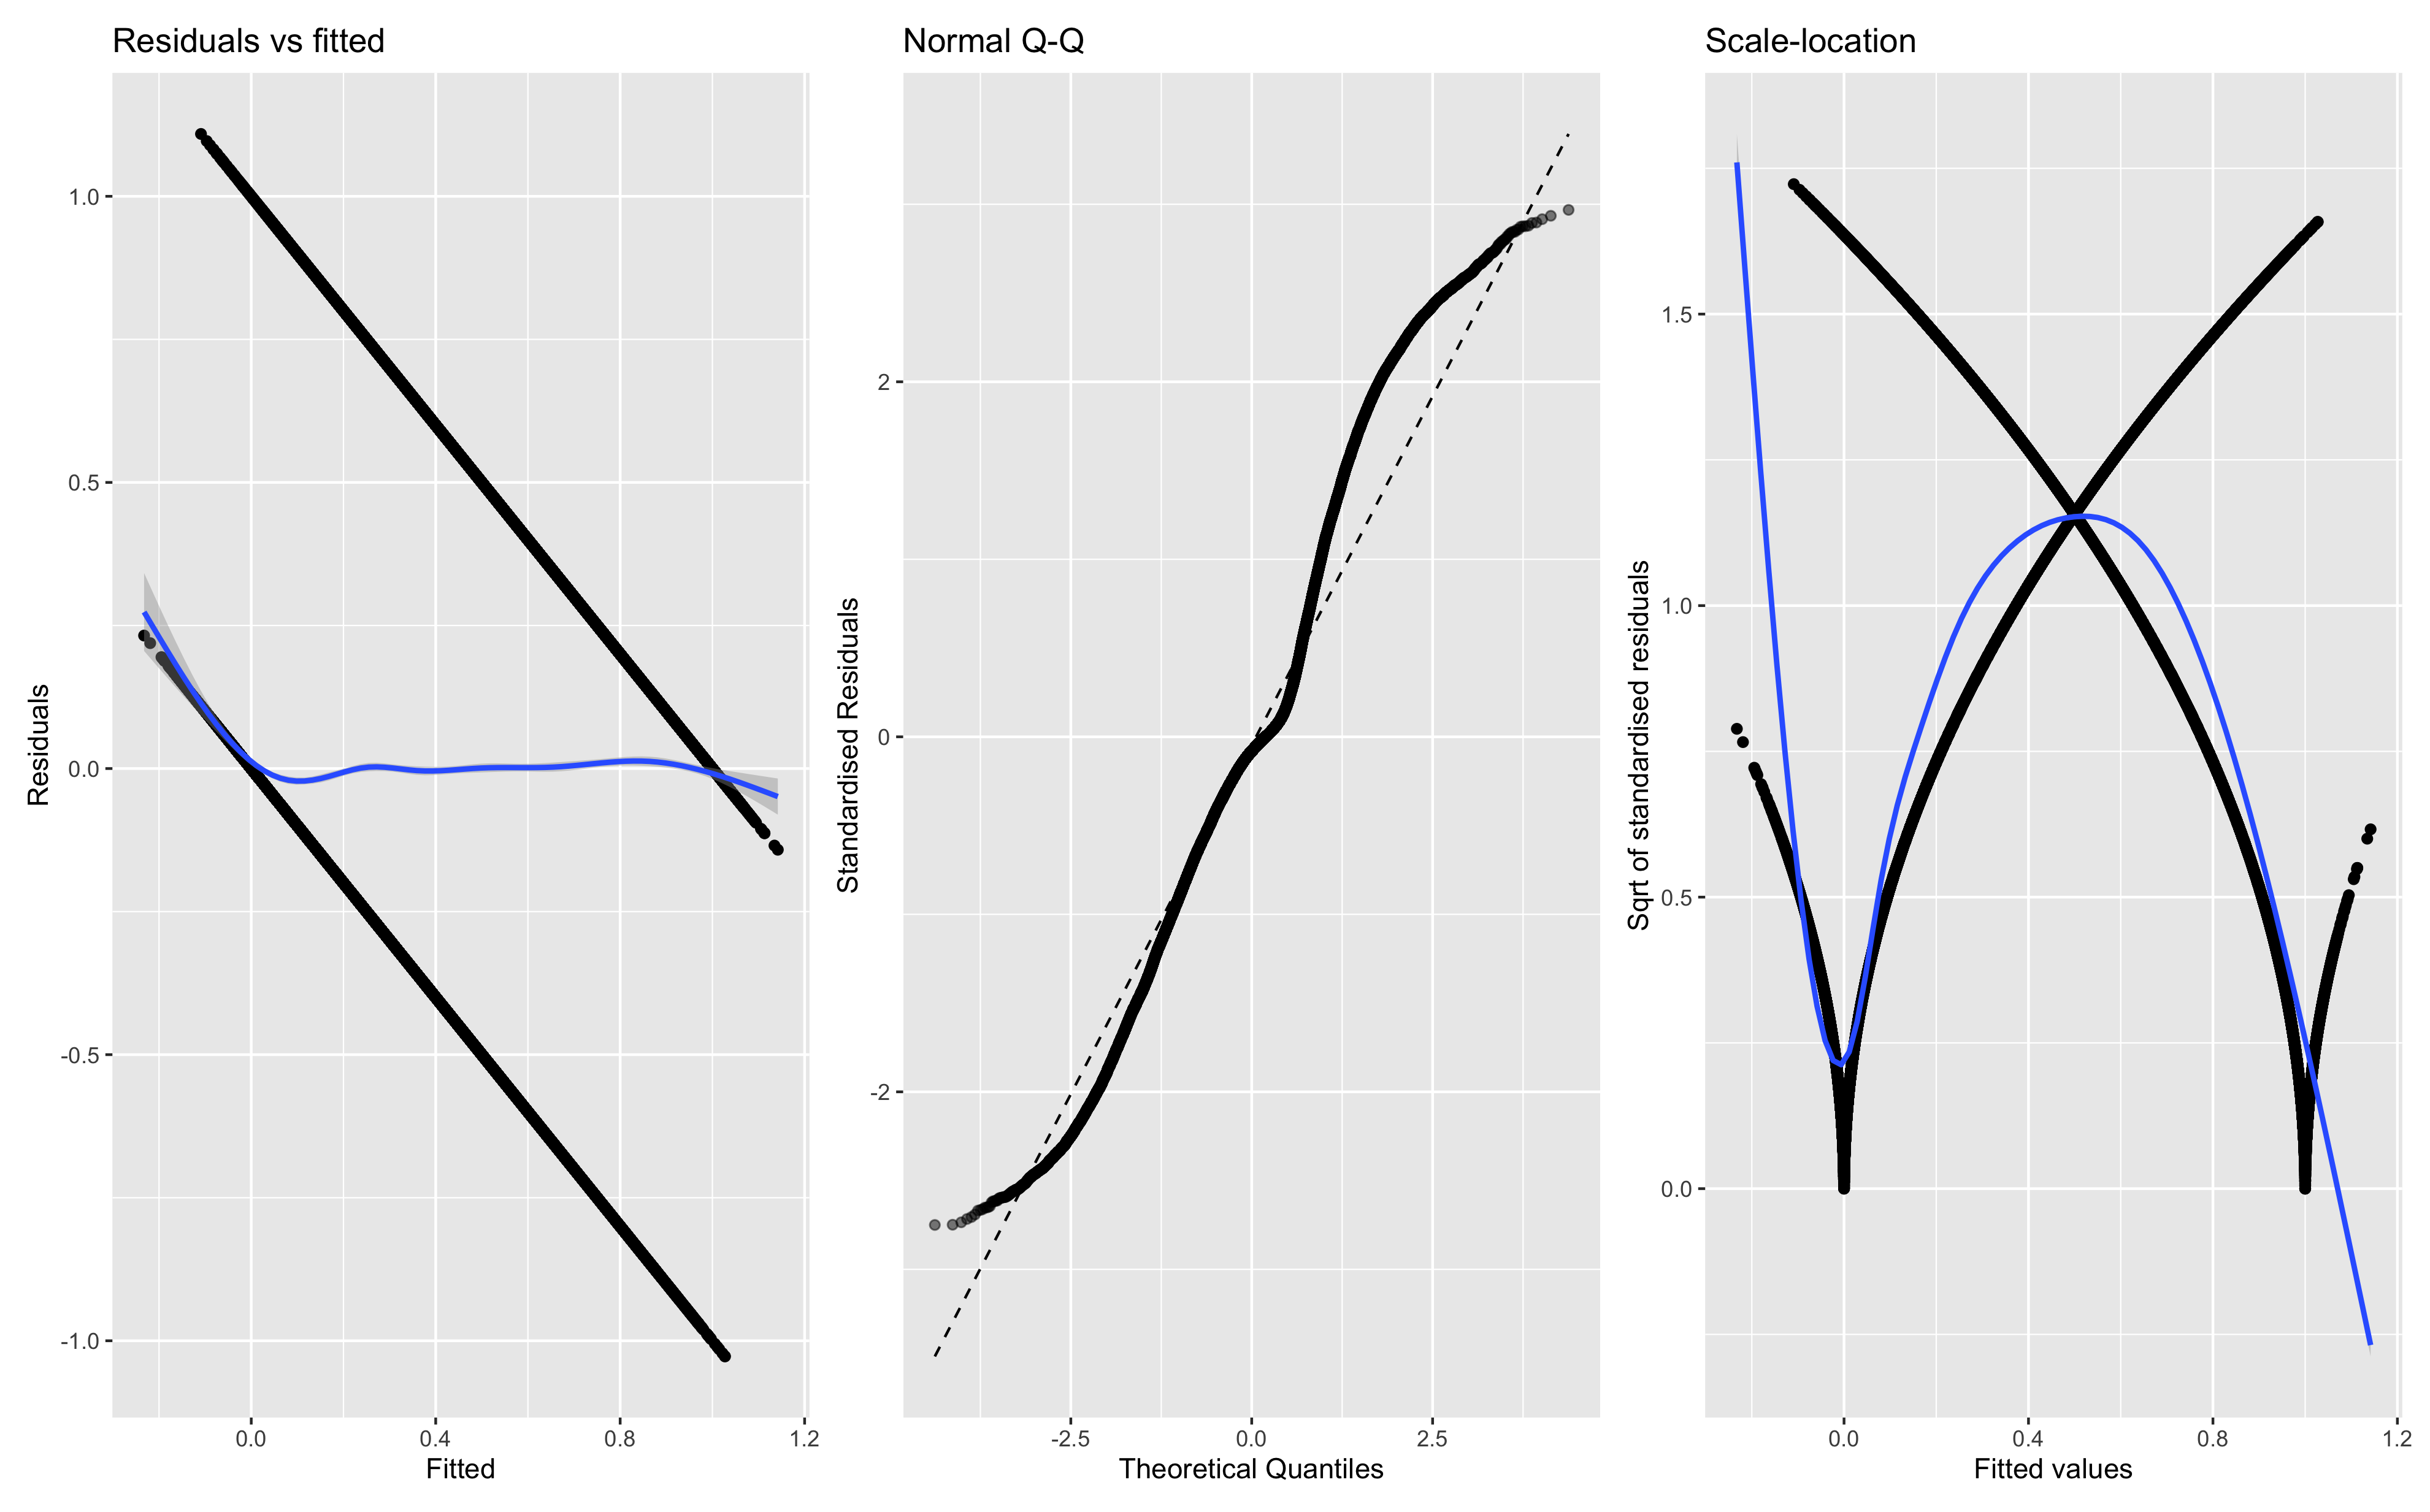
\includegraphics[width=0.9\textwidth]{\figdir/diagnostics.png}
%     \end{center}
% \end{figure}

% \newpage
% \begin{figure}[H]
%     \caption{Entropy and unique tags}
%     \label{fig:entropy_tag_vs_nunique}
%     \begin{center}
%         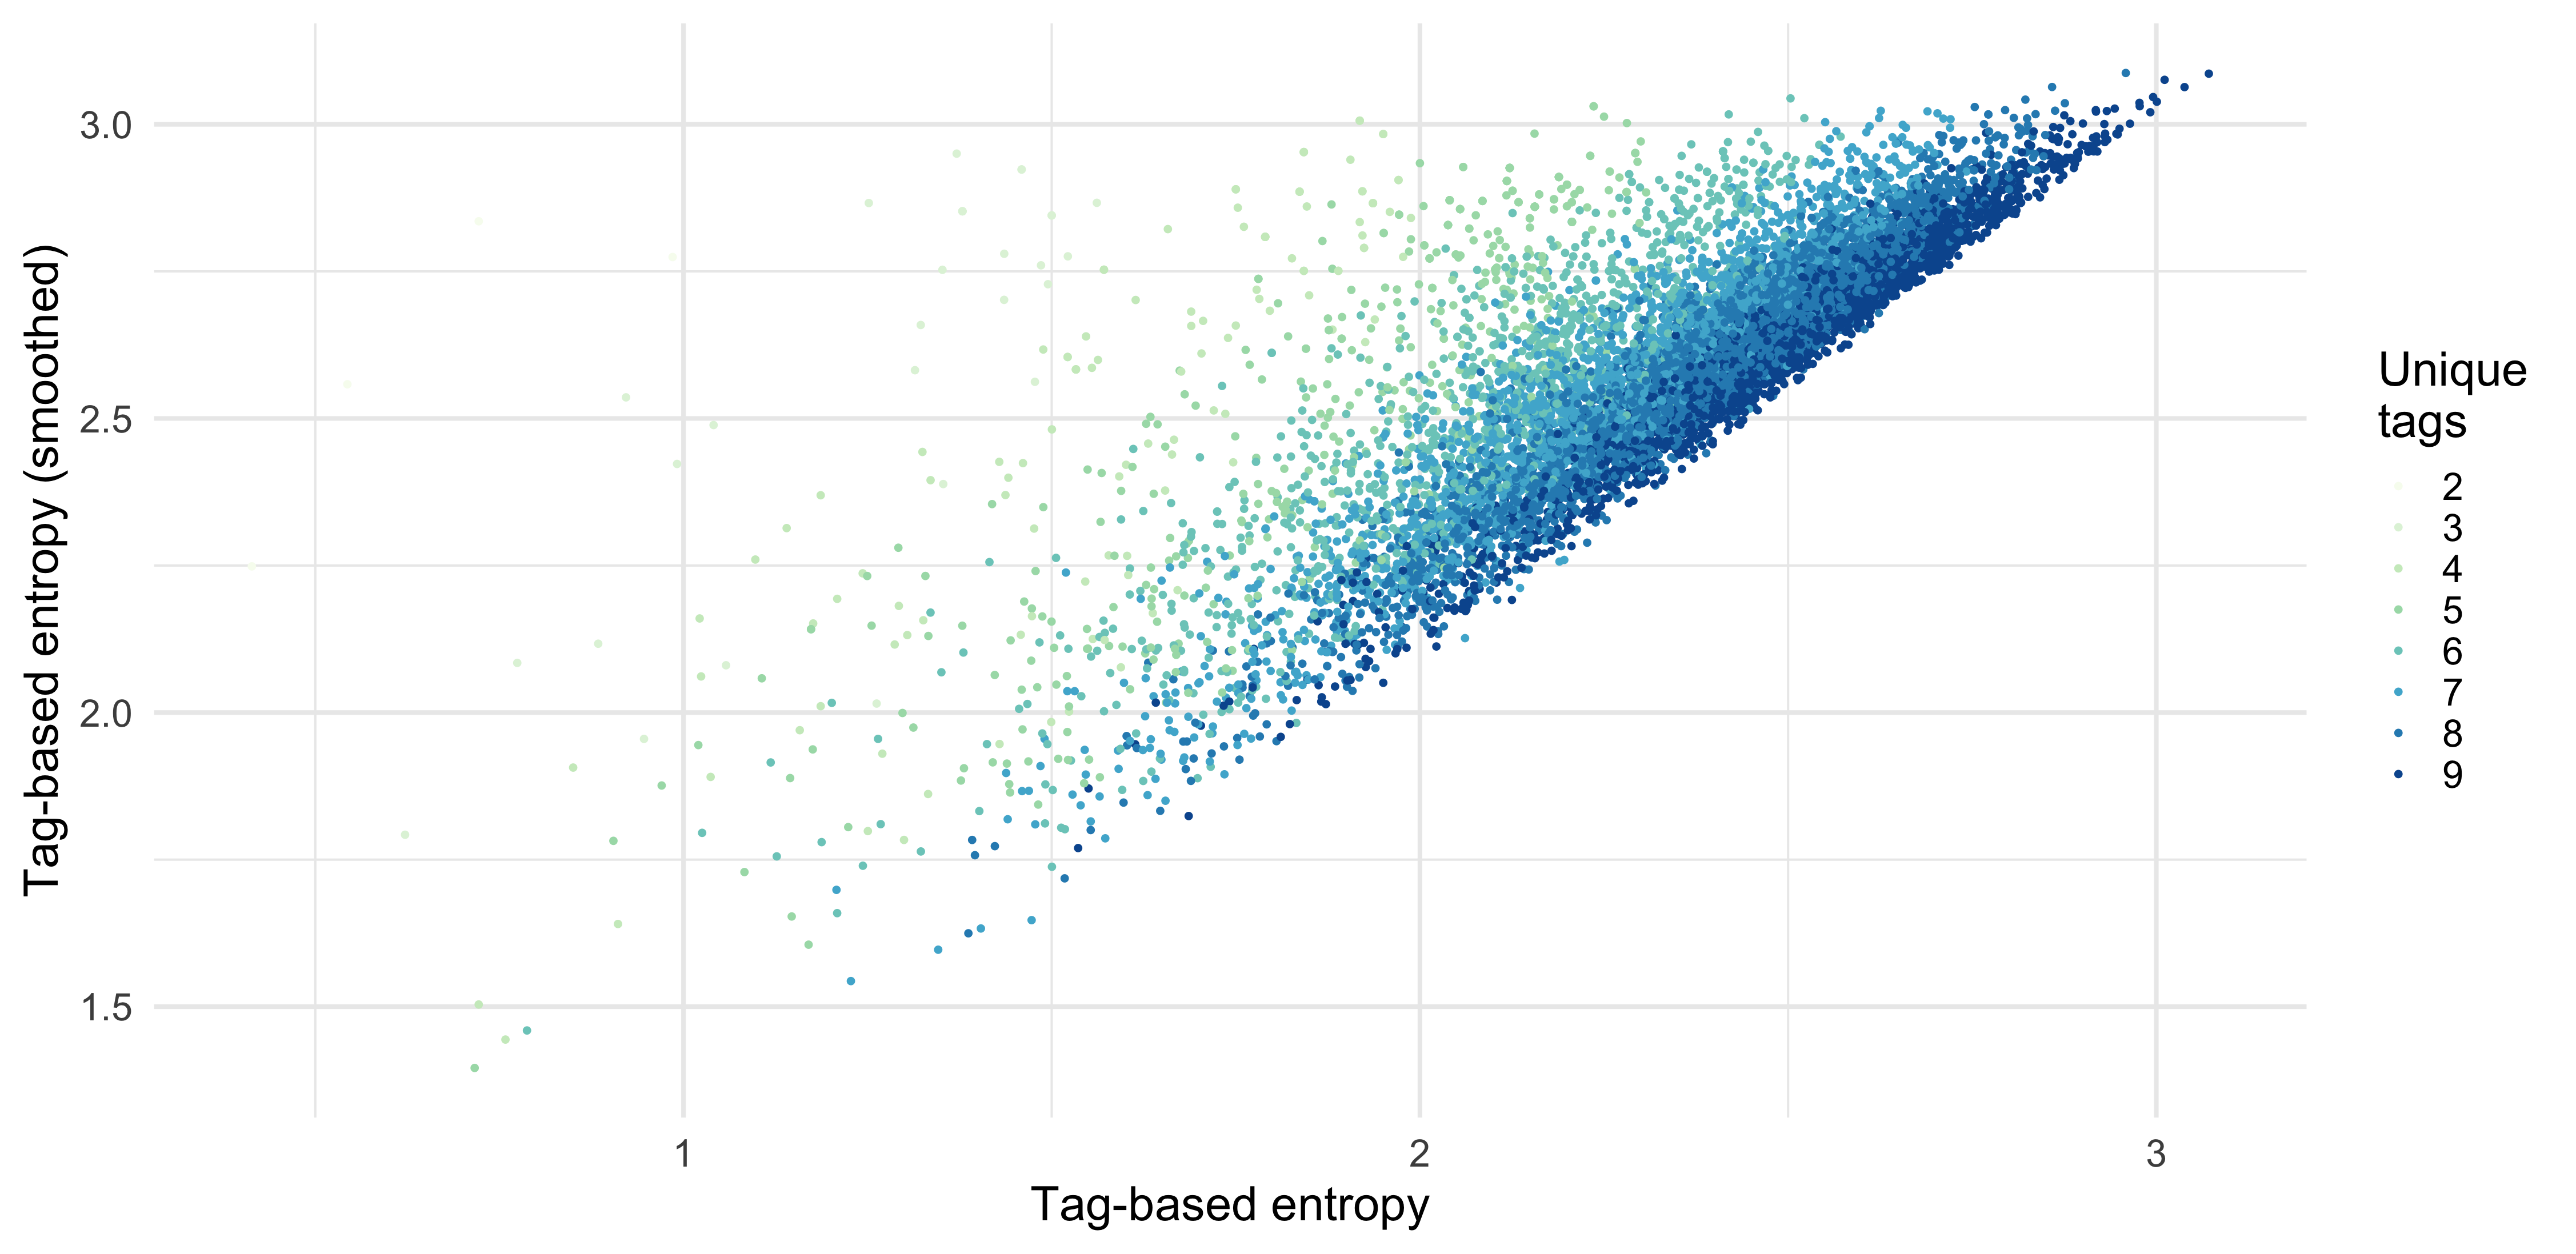
\includegraphics[width=0.9\textwidth]{\figdir/entropy_tag_vs_nunique.png}
%     \end{center}
% \end{figure}



\end{document}
